	\documentclass{article}
\usepackage[colorlinks,citecolor=blue,urlcolor=blue]{hyperref}

\def\bbdot{\dot{\bb}}
\def\bgdot{\dot{\bg}}
\def\gdot{\dot{g}}
\def\ccdot{\dot{c}}
\def\adot{\dot{\ba}}
\def\bdot{\dot{\bb}}
\def\tdot{\dot{\bt}}
\def\tdd{\ddot{t}}
\def\addd{\ddot{a}}
\def\bdd{\ddot{b}}
\def\thetadot{\dot{\btheta}}
\def\covhat{\widehat{\cov}}
\def\siv{_{\text{IV}}}
\def\spp{_{\text{PP}}}
\def\sat{_{\text{AT}}}
\def\stsls{_{\text{TSLS}}}
\def\sps{_{\text{PS}}}
\def\saps{_{\text{APS}}}
\def\xpp{X\spp}



\usepackage[margin=1in]{geometry}
\usepackage{lmodern}
\usepackage{amsmath}               
\usepackage{graphicx}

\usepackage[T1]{fontenc}
\title{Synthetic instrumental variable estimation}
\RequirePackage{amsthm,amsmath,geometry,amsfonts}
\RequirePackage{natbib}
\usepackage[utf8]{inputenc}
\usepackage[english]{babel}
\usepackage{centernot}
%Last Modified : Time-stamp: <02/28/05 4pm tcai>

%%%%%%%%%%%%%%%%%%%%%%%%%%%%%%%%%%%%%%%%%%%%%%
%                                            %
%        GrandMacros.tex                     %
%                                            %
%  A file containing all non-colour LaTeX    %
%  macros used by M.P. Wand                  %
%                                            %
%     Last changed: 17th July, 2000          %
%                                            %
%%%%%%%%%%%%%%%%%%%%%%%%%%%%%%%%%%%%%%%%%%%%%%
%
% Conventions (for most current macros):
%
% \ba        <-->  bold-faced a
% \ahat      <-->  hatted a
% \atilde    <-->  tilded a
% \abar      <-->  barred a
% \asc       <-->  script a
% \aarrow    <-->  arrowed a
% \smbalpha  <-->  small bold-faced alpha
%
%%%%%%%%%%%%%%%%%%%%%%%%%%
%  Bold Digits           %
%%%%%%%%%%%%%%%%%%%%%%%%%%
%
%
\def\bzero{{\bf 0}}
\def\bone{{\bf 1}}
%
%
%%%%%%%%%%%%%%%%%%%%%%%%%%
%  Bold Roman Letters    %
%%%%%%%%%%%%%%%%%%%%%%%%%%
%
%
\def\ba{{\mbox{\boldmath$a$}}}
\def\bb{{\bf b}}
\def\bc{{\bf c}}
\def\bd{{\bf d}}
\def\be{{\bf e}}
\def\bdf{{\bf f}}
\def\bg{{\mbox{\boldmath$g$}}}
\def\bh{{\bf h}}
\def\bi{{\bf i}}
\def\bj{{\bf j}}
\def\bk{{\bf k}}
\def\bl{{\bf l}}
\def\bm{{\bf m}}
\def\bn{{\bf n}}
\def\bo{{\bf o}}
\def\bp{{\bf p}}
\def\bq{{\bf q}}
\def\br{{\bf r}}
\def\bs{{\bf s}}
\def\bt{{\bf t}}
\def\bu{{\bf u}}
\def\bv{{\bf v}}
\def\bw{{\bf w}}
\def\bx{{\bf x}}
\def\by{{\bf y}}
\def\bz{{\bf z}}
\def\bA{{\bf A}}
\def\bB{{\bf B}}
\def\bC{{\bf C}}
\def\bD{{\bf D}}
\def\bE{{\bf E}}
\def\bF{{\bf F}}
\def\bG{{\bf G}}
\def\bH{{\bf H}}
\def\bI{{\bf I}}
\def\bJ{{\bf J}}
\def\bK{{\bf K}}
\def\bL{{\bf L}}
\def\bM{{\bf M}}
\def\bN{{\bf N}}
\def\bO{{\bf O}}
\def\bP{{\bf P}}
\def\bQ{{\bf Q}}
\def\bR{{\bf R}}
\def\bS{{\bf S}}
\def\bT{{\bf T}}
\def\bU{{\bf U}}
\def\bV{{\bf V}}
\def\bW{{\bf W}}
\def\bX{{\bf X}}
\def\bY{{\bf Y}}
\def\bZ{{\bf Z}}
\def\smbZ{\scriptstyle{\bf Z}}
\def\smM{\scriptstyle{M}}
\def\smN{\scriptstyle{N}}
\def\smbT{\scriptstyle{\bf T}}
%
%
%%%%%%%%%%%%%%%%%%%%%%%%%%
%  Bold Greek Letters    %
%%%%%%%%%%%%%%%%%%%%%%%%%%
%
%
\def\thick#1{\hbox{\rlap{$#1$}\kern0.25pt\rlap{$#1$}\kern0.25pt$#1$}}
\def\balpha{\boldsymbol{\alpha}}
\def\bbeta{\boldsymbol{\beta}}
\def\bgamma{\boldsymbol{\gamma}}
\def\bdelta{\boldsymbol{\delta}}
\def\bepsilon{\boldsymbol{\epsilon}}
\def\bvarepsilon{\boldsymbol{\varepsilon}}
\def\bzeta{\boldsymbol{\zeta}}
\def\bdeta{\boldsymbol{\eta}}
\def\btheta{\boldsymbol{\theta}}
\def\biota{\boldsymbol{\iota}}
\def\bkappa{\boldsymbol{\kappa}}
\def\blambda{\boldsymbol{\lambda}}
\def\bmu{\boldsymbol{\mu}}
\def\bnu{\boldsymbol{\nu}}
\def\bxi{\boldsymbol{\xi}}
\def\bomicron{\boldsymbol{\omicron}}
\def\bpi{\boldsymbol{\pi}}
\def\brho{\boldsymbol{\rho}}
\def\bsigma{\boldsymbol{\sigma}}
\def\btau{\boldsymbol{\tau}}
\def\bupsilon{\boldsymbol{\upsilon}}
\def\bphi{\boldsymbol{\phi}}
\def\bchi{\boldsymbol{\chi}}
\def\bpsi{\boldsymbol{\psi}}
\def\bomega{\boldsymbol{\omega}}
\def\bAlpha{\boldsymbol{\Alpha}}
\def\bBeta{\boldsymbol{\Beta}}
\def\bGamma{\boldsymbol{\Gamma}}
\def\bDelta{\boldsymbol{\Delta}}
\def\bEpsilon{\boldsymbol{\Epsilon}}
\def\bZeta{\boldsymbol{\Zeta}}
\def\bEta{\boldsymbol{\Eta}}
\def\bTheta{\boldsymbol{\Theta}}
\def\bIota{\boldsymbol{\Iota}}
\def\bKappa{\boldsymbol{\Kappa}}
\def\bLambda{{\boldsymbol{\Lambda}}}
\def\bMu{\boldsymbol{\Mu}}
\def\bNu{\boldsymbol{\Nu}}
\def\bXi{\boldsymbol{\Xi}}
\def\bOmicron{\boldsymbol{\Omicron}}
\def\bPi{\boldsymbol{\Pi}}
\def\bRho{\boldsymbol{\Rho}}
\def\bSigma{\boldsymbol{\Sigma}}
\def\bTau{\boldsymbol{\Tau}}
\def\bUpsilon{\boldsymbol{\Upsilon}}
\def\bPhi{\boldsymbol{\Phi}}
\def\bChi{\boldsymbol{\Chi}}
\def\bPsi{\boldsymbol{\Psi}}
\def\bOmega{\boldsymbol{\Omega}}
%
%
%
%%%%%%%%%%%%%%%%%%%%%%%%%%%%%%%%
%  Small Bold Greek Letters    %
%%%%%%%%%%%%%%%%%%%%%%%%%%%%%%%%
\def\smalpha{{{\scriptstyle{\alpha}}}}
\def\smbeta{{{\scriptstyle{\beta}}}}
\def\smgamma{{{\scriptstyle{\gamma}}}}
\def\smdelta{{{\scriptstyle{\delta}}}}
\def\smepsilon{{{\scriptstyle{\epsilon}}}}
\def\smvarepsilon{{{\scriptstyle{\varepsilon}}}}
\def\smzeta{{{\scriptstyle{\zeta}}}}
\def\smdeta{{{\scriptstyle{\eta}}}}
\def\smtheta{{{\scriptstyle{\theta}}}}
\def\smiota{{{\scriptstyle{\iota}}}}
\def\smkappa{{{\scriptstyle{\kappa}}}}
\def\smlambda{{{\scriptstyle{\lambda}}}}
\def\smmu{{{\scriptstyle{\mu}}}}
\def\smnu{{{\scriptstyle{\nu}}}}
\def\smxi{{{\scriptstyle{\xi}}}}
\def\smomicron{{{\scriptstyle{\omicron}}}}
\def\smpi{{{\scriptstyle{\pi}}}}
\def\smrho{{{\scriptstyle{\rho}}}}
\def\smsigma{{{\scriptstyle{\sigma}}}}
\def\smtau{{{\scriptstyle{\tau}}}}
\def\smupsilon{{{\scriptstyle{\upsilon}}}}
\def\smphi{{{\scriptstyle{\phi}}}}
\def\smchi{{{\scriptstyle{\chi}}}}
\def\smpsi{{{\scriptstyle{\psi}}}}
\def\smomega{{{\scriptstyle{\omega}}}}
\def\smAlpha{{{\scriptstyle{\Alpha}}}}
\def\smBeta{{{\scriptstyle{\Beta}}}}
\def\smGamma{{{\scriptstyle{\Gamma}}}}
\def\smDelta{{{\scriptstyle{\Delta}}}}
\def\smEpsilon{{{\scriptstyle{\Epsilon}}}}
\def\smZeta{{{\scriptstyle{\Zeta}}}}
\def\smEta{{{\scriptstyle{\Eta}}}}
\def\smTheta{{{\scriptstyle{\Theta}}}}
\def\smIota{{{\scriptstyle{\Iota}}}}
\def\smKappa{{{\scriptstyle{\Kappa}}}}
\def\smLambda{{{\scriptstyle{\Lambda}}}}
\def\smMu{{{\scriptstyle{\Mu}}}}
\def\smNu{{{\scriptstyle{\Nu}}}}
\def\smXi{{{\scriptstyle{\Xi}}}}
\def\smOmicron{{{\scriptstyle{\Omicron}}}}
\def\smPi{{{\scriptstyle{\Pi}}}}
\def\smRho{{{\scriptstyle{\Rho}}}}
\def\smSigma{{{\scriptstyle{\Sigma}}}}
\def\smTau{{{\scriptstyle{\Tau}}}}
\def\smUpsilon{{{\scriptstyle{\Upsilon}}}}
\def\smPhi{{{\scriptstyle{\Phi}}}}
\def\smChi{{{\scriptstyle{\Chi}}}}
\def\smPsi{{{\scriptstyle{\Psi}}}}
\def\smOmega{{{\scriptstyle{\Omega}}}}
%
%

%
%%%%%%%%%%%%%%%%%%%%%%%%%%%%%%%%
%  Small Bold Greek Letters    %
%%%%%%%%%%%%%%%%%%%%%%%%%%%%%%%%
\def\smbalpha{\boldsymbol{{\scriptstyle{\alpha}}}}
\def\smbbeta{\boldsymbol{{\scriptstyle{\beta}}}}
\def\smbgamma{\boldsymbol{{\scriptstyle{\gamma}}}}
\def\smbdelta{\boldsymbol{{\scriptstyle{\delta}}}}
\def\smbepsilon{\boldsymbol{{\scriptstyle{\epsilon}}}}
\def\smbvarepsilon{\boldsymbol{{\scriptstyle{\varepsilon}}}}
\def\smbzeta{\boldsymbol{{\scriptstyle{\zeta}}}}
\def\smbdeta{\boldsymbol{{\scriptstyle{\eta}}}}
\def\smbtheta{\boldsymbol{{\scriptstyle{\theta}}}}
\def\smbiota{\boldsymbol{{\scriptstyle{\iota}}}}
\def\smbkappa{\boldsymbol{{\scriptstyle{\kappa}}}}
\def\smblambda{\boldsymbol{{\scriptstyle{\lambda}}}}
\def\smbmu{\boldsymbol{{\scriptstyle{\mu}}}}
\def\smbnu{\boldsymbol{{\scriptstyle{\nu}}}}
\def\smbxi{\boldsymbol{{\scriptstyle{\xi}}}}
\def\smbomicron{\boldsymbol{{\scriptstyle{\omicron}}}}
\def\smbpi{\boldsymbol{{\scriptstyle{\pi}}}}
\def\smbrho{\boldsymbol{{\scriptstyle{\rho}}}}
\def\smbsigma{\boldsymbol{{\scriptstyle{\sigma}}}}
\def\smbtau{\boldsymbol{{\scriptstyle{\tau}}}}
\def\smbupsilon{\boldsymbol{{\scriptstyle{\upsilon}}}}
\def\smbphi{\boldsymbol{{\scriptstyle{\phi}}}}
\def\smbchi{\boldsymbol{{\scriptstyle{\chi}}}}
\def\smbpsi{\boldsymbol{{\scriptstyle{\psi}}}}
\def\smbomega{\boldsymbol{{\scriptstyle{\omega}}}}
\def\smbAlpha{\boldsymbol{{\scriptstyle{\Alpha}}}}
\def\smbBeta{\boldsymbol{{\scriptstyle{\Beta}}}}
\def\smbGamma{\boldsymbol{{\scriptstyle{\Gamma}}}}
\def\smbDelta{\boldsymbol{{\scriptstyle{\Delta}}}}
\def\smbEpsilon{\boldsymbol{{\scriptstyle{\Epsilon}}}}
\def\smbZeta{\boldsymbol{{\scriptstyle{\Zeta}}}}
\def\smbEta{\boldsymbol{{\scriptstyle{\Eta}}}}
\def\smbTheta{\boldsymbol{{\scriptstyle{\Theta}}}}
\def\smbIota{\boldsymbol{{\scriptstyle{\Iota}}}}
\def\smbKappa{\boldsymbol{{\scriptstyle{\Kappa}}}}
\def\smbLambda{\boldsymbol{{\scriptstyle{\Lambda}}}}
\def\smbMu{\boldsymbol{{\scriptstyle{\Mu}}}}
\def\smbNu{\boldsymbol{{\scriptstyle{\Nu}}}}
\def\smbXi{\boldsymbol{{\scriptstyle{\Xi}}}}
\def\smbOmicron{\boldsymbol{{\scriptstyle{\Omicron}}}}
\def\smbPi{\boldsymbol{{\scriptstyle{\Pi}}}}
\def\smbRho{\boldsymbol{{\scriptstyle{\Rho}}}}
\def\smbSigma{\boldsymbol{{\scriptstyle{\Sigma}}}}
\def\smbTau{\boldsymbol{{\scriptstyle{\Tau}}}}
\def\smbUpsilon{\boldsymbol{{\scriptstyle{\Upsilon}}}}
\def\smbPhi{\boldsymbol{{\scriptstyle{\Phi}}}}
\def\smbChi{\boldsymbol{{\scriptstyle{\Chi}}}}
\def\smbPsi{\boldsymbol{{\scriptstyle{\Psi}}}}
\def\smbOmega{\boldsymbol{{\scriptstyle{\Omega}}}}
%
%
%%%%%%%%%%%%%%%%%%%%%%%%%%
%  Hatted Roman Letters  %
%%%%%%%%%%%%%%%%%%%%%%%%%%
%
%
\def\ahat{{\widehat a}}
\def\bhat{{\widehat b}}
\def\chat{{\widehat c}}
\def\dhat{{\widehat d}}
\def\ehat{{\widehat e}}
\def\fhat{{\widehat f}}
\def\ghat{{\widehat g}}
\def\hhat{{\widehat h}}
\def\ihat{{\widehat i}}
\def\jhat{{\widehat j}}
\def\khat{{\widehat k}}
\def\lhat{{\widehat l}}
\def\mhat{{\widehat m}}
\def\nhat{{\widehat n}}
\def\ohat{{\widehat o}}
\def\phat{{\widehat p}}
\def\qhat{{\widehat q}}
\def\rhat{{\widehat r}}
\def\shat{{\widehat s}}
\def\that{{\widehat t}}
\def\uhat{{\widehat u}}
\def\vhat{{\widehat v}}
\def\what{{\widehat w}}
\def\xhat{{\widehat x}}
\def\yhat{{\widehat y}}
\def\zhat{{\widehat z}}
\def\Ahat{{\widehat A}}
\def\Bhat{{\widehat B}}
\def\Chat{{\widehat C}}
\def\Dhat{{\widehat D}}
\def\Ehat{{\widehat E}}
\def\Fhat{{\widehat F}}
\def\Ghat{{\widehat G}}
\def\Hhat{{\widehat H}}
\def\Ihat{{\widehat I}}
\def\Jhat{{\widehat J}}
\def\Khat{{\widehat K}}
\def\Lhat{{\widehat L}}
\def\Mhat{{\widehat M}}
\def\Nhat{{\widehat N}}
\def\Ohat{{\widehat O}}
\def\Phat{{\widehat P}}
\def\Qhat{{\widehat Q}}
\def\Rhat{{\widehat R}}
\def\Shat{{\widehat S}}
\def\That{{\widehat T}}
\def\Uhat{{\widehat U}}
\def\Vhat{{\widehat V}}
\def\What{{\widehat W}}
\def\Xhat{{\widehat X}}
\def\Yhat{{\widehat Y}}
\def\Zhat{{\widehat Z}}
%
%%%%%%%%%%%%%%%%%%%%%%%%%%
%  Tilded Roman Letters  %
%%%%%%%%%%%%%%%%%%%%%%%%%%
%
%
\def\atilde{{\widetilde a}}
\def\btilde{{\widetilde b}}
\def\ctilde{{\widetilde c}}
\def\dtilde{{\widetilde d}}
\def\etilde{{\widetilde e}}
\def\ftilde{{\widetilde f}}
\def\gtilde{{\widetilde g}}
\def\htilde{{\widetilde h}}
\def\itilde{{\widetilde i}}
\def\jtilde{{\widetilde j}}
\def\ktilde{{\widetilde k}}
\def\ltilde{{\widetilde l}}
\def\mtilde{{\widetilde m}}
\def\ntilde{{\widetilde n}}
\def\otilde{{\widetilde o}}
\def\ptilde{{\widetilde p}}
\def\qtilde{{\widetilde q}}
\def\rtilde{{\widetilde r}}
\def\stilde{{\widetilde s}}
\def\ttilde{{\widetilde t}}
\def\utilde{{\widetilde u}}
\def\vtilde{{\widetilde v}}
\def\wtilde{{\widetilde w}}
\def\xtilde{{\widetilde x}}
\def\ytilde{{\widetilde y}}
\def\ztilde{{\widetilde z}}
\def\Atilde{{\widetilde A}}
\def\Btilde{{\widetilde B}}
\def\Ctilde{{\widetilde C}}
\def\Dtilde{{\widetilde D}}
\def\Etilde{{\widetilde E}}
\def\Ftilde{{\widetilde F}}
\def\Gtilde{{\widetilde G}}
\def\Htilde{{\widetilde H}}
\def\Itilde{{\widetilde I}}
\def\Jtilde{{\widetilde J}}
\def\Ktilde{{\widetilde K}}
\def\Ltilde{{\widetilde L}}
\def\Mtilde{{\widetilde M}}
\def\Ntilde{{\widetilde N}}
\def\Otilde{{\widetilde O}}
\def\Ptilde{{\widetilde P}}
\def\Qtilde{{\widetilde Q}}
\def\Rtilde{{\widetilde R}}
\def\Stilde{{\widetilde S}}
\def\Ttilde{{\widetilde T}}
\def\Utilde{{\widetilde U}}
\def\Vtilde{{\widetilde V}}
\def\Wtilde{{\widetilde W}}
\def\Xtilde{{\widetilde X}}
\def\Ytilde{{\widetilde Y}}
\def\Ztilde{{\widetilde Z}}
%
%
%%%%%%%%%%%%%%%%%%%%%%%%%%%%%%%%%%%%
%  Hatted Bold-faced Roman Letters %
%%%%%%%%%%%%%%%%%%%%%%%%%%%%%%%%%%%%
%
%
\def\bahat{{\widehat \ba}}
\def\bbhat{{\widehat \bb}}
\def\bchat{{\widehat \bc}}
\def\bdhat{{\widehat \bd}}
\def\behat{{\widehat \be}}
\def\bfhat{{\widehat \bf}}
\def\bghat{{\widehat \bg}}
\def\bhhat{{\widehat \bh}}
\def\bihat{{\widehat \bi}}
\def\bjhat{{\widehat \bj}}
\def\bkhat{{\widehat \bk}}
\def\blhat{{\widehat \bl}}
\def\bmhat{{\widehat \bm}}
\def\bnhat{{\widehat \bn}}
\def\bohat{{\widehat \bo}}
\def\bphat{{\widehat \bp}}
\def\bqhat{{\widehat \bq}}
\def\brhat{{\widehat \br}}
\def\bshat{{\widehat \bs}}
\def\bthat{{\widehat \bt}}
\def\buhat{{\widehat \bu}}
\def\bvhat{{\widehat \bv}}
\def\bwhat{{\widehat \bw}}
\def\bxhat{{\widehat \bx}}
\def\byhat{{\widehat \by}}
\def\bzhat{{\widehat \bz}}
\def\bAhat{{\widehat \bA}}
\def\bBhat{{\widehat \bB}}
\def\bChat{{\widehat \bC}}
\def\bDhat{{\widehat \bD}}
\def\bEhat{{\widehat \bE}}
\def\bFhat{{\widehat \bF}}
\def\bGhat{{\widehat \bG}}
\def\bHhat{{\widehat \bH}}
\def\bIhat{{\widehat \bI}}
\def\bJhat{{\widehat \bJ}}
\def\bKhat{{\widehat \bK}}
\def\bLhat{{\widehat \bL}}
\def\bMhat{{\widehat \bM}}
\def\bNhat{{\widehat \bN}}
\def\bOhat{{\widehat \bO}}
\def\bPhat{{\widehat \bP}}
\def\bQhat{{\widehat \bQ}}
\def\bRhat{{\widehat \bR}}
\def\bShat{{\widehat \bS}}
\def\bThat{{\widehat \bT}}
\def\bUhat{{\widehat \bU}}
\def\bVhat{{\widehat \bV}}
\def\bWhat{{\widehat \bW}}
\def\bXhat{{\widehat \bX}}
\def\bYhat{{\widehat \bY}}
\def\bZhat{{\widehat \bZ}}
%
%
%
%%%%%%%%%%%%%%%%%%%%%%%%%%%%%%%%%%%%
%  Tilded Bold-faced Roman Letters %
%%%%%%%%%%%%%%%%%%%%%%%%%%%%%%%%%%%%
%
%
\def\batilde{{\widetilde \ba}}
\def\bbtilde{{\widetilde \bb}}
\def\bctilde{{\widetilde \bc}}
\def\bdtilde{{\widetilde \bd}}
\def\betilde{{\widetilde \be}}
\def\bftilde{{\widetilde \bf}}
\def\bgtilde{{\widetilde \bg}}
\def\bhtilde{{\widetilde \bh}}
\def\bitilde{{\widetilde \bi}}
\def\bjtilde{{\widetilde \bj}}
\def\bktilde{{\widetilde \bk}}
\def\bltilde{{\widetilde \bl}}
\def\bmtilde{{\widetilde \bm}}
\def\bntilde{{\widetilde \bn}}
\def\botilde{{\widetilde \bo}}
\def\bptilde{{\widetilde \bp}}
\def\bqtilde{{\widetilde \bq}}
\def\brtilde{{\widetilde \br}}
\def\bstilde{{\widetilde \bs}}
\def\bttilde{{\widetilde \bt}}
\def\butilde{{\widetilde \bu}}
\def\bvtilde{{\widetilde \bv}}
\def\bwtilde{{\widetilde \bw}}
\def\bxtilde{{\widetilde \bx}}
\def\bytilde{{\widetilde \by}}
\def\bztilde{{\widetilde \bz}}
\def\bAtilde{{\widetilde \bA}}
\def\bBtilde{{\widetilde \bB}}
\def\bCtilde{{\widetilde \bC}}
\def\bDtilde{{\widetilde \bD}}
\def\bEtilde{{\widetilde \bE}}
\def\bFtilde{{\widetilde \bF}}
\def\bGtilde{{\widetilde \bG}}
\def\bHtilde{{\widetilde \bH}}
\def\bItilde{{\widetilde \bI}}
\def\bJtilde{{\widetilde \bJ}}
\def\bKtilde{{\widetilde \bK}}
\def\bLtilde{{\widetilde \bL}}
\def\bMtilde{{\widetilde \bM}}
\def\bNtilde{{\widetilde \bN}}
\def\bOtilde{{\widetilde \bO}}
\def\bPtilde{{\widetilde \bP}}
\def\bQtilde{{\widetilde \bQ}}
\def\bRtilde{{\widetilde \bR}}
\def\bStilde{{\widetilde \bS}}
\def\bTtilde{{\widetilde \bT}}
\def\bUtilde{{\widetilde \bU}}
\def\bVtilde{{\widetilde \bV}}
\def\bWtilde{{\widetilde \bW}}
\def\bXtilde{{\widetilde \bX}}
\def\bYtilde{{\widetilde \bY}}
\def\bZtilde{{\widetilde \bZ}}
%
%
%
%
%%%%%%%%%%%%%%%%%%%%%%%%%%
%  Hatted Greek Letters  %
%%%%%%%%%%%%%%%%%%%%%%%%%%
%
%
\def\alphahat{{\widehat\alpha}}
\def\betahat{{\widehat\beta}}
\def\gammahat{{\widehat\gamma}}
\def\deltahat{{\widehat\delta}}
\def\epsilonhat{{\widehat\epsilon}}
\def\varepsilonhat{{\widehat\varepsilon}}
\def\zetahat{{\widehat\zeta}}
\def\etahat{{\widehat\eta}}
\def\thetahat{{\widehat\theta}}
\def\iotahat{{\widehat\iota}}
\def\kappahat{{\widehat\kappa}}
\def\lambdahat{{\widehat\lambda}}
\def\muhat{{\widehat\mu}}
\def\nuhat{{\widehat\nu}}
\def\xihat{{\widehat\xi}}
\def\omicronhat{{\widehat\omicron}}
\def\pihat{{\widehat\pi}}
\def\rhohat{{\widehat\rho}}
\def\sigmahat{{\widehat\sigma}}
\def\tauhat{{\widehat\tau}}
\def\upsilonhat{{\widehat\upsilon}}
\def\phihat{{\widehat\phi}}
\def\chihat{{\widehat\chi}}
\def\psihat{{\widehat\psi}}
\def\omegahat{{\widehat\omega}}
\def\Alphahat{{\widehat\Alpha}}
\def\Betahat{{\widehat\Beta}}
\def\Gammahat{{\widehat\Gamma}}
\def\Deltahat{{\widehat\Delta}}
\def\Epsilonhat{{\widehat\Epsilon}}
\def\Zetahat{{\widehat\Zeta}}
\def\Etahat{{\widehat\Eta}}
\def\Thetahat{{\widehat\Theta}}
\def\Iotahat{{\widehat\Iota}}
\def\Kappahat{{\widehat\Kappa}}
\def\Lambdahat{{\widehat\Lambda}}
\def\Muhat{{\widehat\Mu}}
\def\Nuhat{{\widehat\Nu}}
\def\Xihat{{\widehat\Xi}}
\def\Omicronhat{{\widehat\Omicron}}
\def\Pihat{{\widehat\Pi}}
\def\Rhohat{{\widehat\Rho}}
\def\Sigmahat{{\widehat\Sigma}}
\def\Tauhat{{\widehat\Tau}}
\def\Upsilonhat{{\widehat\Upsilon}}
\def\Phihat{{\widehat\Phi}}
\def\Chihat{{\widehat\Chi}}
\def\Psihat{{\widehat\Psi}}
\def\Omegahat{{\widehat\Omega}}
%
%
%
%%%%%%%%%%%%%%%%%%%%%%%%%%
%  Tilded Greek Letters  %
%%%%%%%%%%%%%%%%%%%%%%%%%%
%
%
\def\alphatilde{{\widetilde\alpha}}
\def\betatilde{{\widetilde\beta}}
\def\gammatilde{{\widetilde\gamma}}
\def\deltatilde{{\widetilde\delta}}
\def\epsilontilde{{\widetilde\epsilon}}
\def\varepsilontilde{{\widetilde\varepsilon}}
\def\zetatilde{{\widetilde\zeta}}
\def\etatilde{{\widetilde\eta}}
\def\thetatilde{{\widetilde\theta}}
\def\iotatilde{{\widetilde\iota}}
\def\kappatilde{{\widetilde\kappa}}
\def\lambdatilde{{\widetilde\lambda}}
\def\mutilde{{\widetilde\mu}}
\def\nutilde{{\widetilde\nu}}
\def\xitilde{{\widetilde\xi}}
\def\omicrontilde{{\widetilde\omicron}}
\def\pitilde{{\widetilde\pi}}
\def\rhotilde{{\widetilde\rho}}
\def\sigmatilde{{\widetilde\sigma}}
\def\tautilde{{\widetilde\tau}}
\def\upsilontilde{{\widetilde\upsilon}}
\def\phitilde{{\widetilde\phi}}
\def\chitilde{{\widetilde\chi}}
\def\psitilde{{\widetilde\psi}}
\def\omegatilde{{\widetilde\omega}}
\def\Alphatilde{{\widetilde\Alpha}}
\def\Betatilde{{\widetilde\Beta}}
\def\Gammatilde{{\widetilde\Gamma}}
\def\Deltatilde{{\widetilde\Delta}}
\def\Epsilontilde{{\widetilde\Epsilon}}
\def\Zetatilde{{\widetilde\Zeta}}
\def\Etatilde{{\widetilde\Eta}}
\def\Thetatilde{{\widetilde\Theta}}
\def\Iotatilde{{\widetilde\Iota}}
\def\Kappatilde{{\widetilde\Kappa}}
\def\Lambdatilde{{\widetilde\Lambda}}
\def\Mutilde{{\widetilde\Mu}}
\def\Nutilde{{\widetilde\Nu}}
\def\Xitilde{{\widetilde\Xi}}
\def\Omicrontilde{{\widetilde\Omicron}}
\def\Pitilde{{\widetilde\Pi}}
\def\Rhotilde{{\widetilde\Rho}}
\def\Sigmatilde{{\widetilde\Sigma}}
\def\Tautilde{{\widetilde\Tau}}
\def\Upsilontilde{{\widetilde\Upsilon}}
\def\Phitilde{{\widetilde\Phi}}
\def\Chitilde{{\widetilde\Chi}}
\def\Psitilde{{\widetilde\Psi}}
\def\Omegatilde{{\widetilde\Omega}}
%
%
%
%
%%%%%%%%%%%%%%%%%%%%%%%%%%%%%%%%%%%%%
%  Hatted Bold-faced Greek Letters  %
%%%%%%%%%%%%%%%%%%%%%%%%%%%%%%%%%%%%%
%
%
\def\balphahat{{\widehat\balpha}}
\def\bbetahat{{\widehat\bbeta}}
\def\bgammahat{{\widehat\bgamma}}
\def\bdeltahat{{\widehat\bdelta}}
\def\bepsilonhat{{\widehat\bepsilon}}
\def\bzetahat{{\widehat\bzeta}}
\def\bdetahat{{\widehat\bdeta}}
\def\bthetahat{{\widehat\btheta}}
\def\biotahat{{\widehat\biota}}
\def\bkappahat{{\widehat\bkappa}}
\def\blambdahat{{\widehat\blambda}}
\def\bmuhat{{\widehat\bmu}}
\def\bnuhat{{\widehat\bnu}}
\def\bxihat{{\widehat\bxi}}
\def\bomicronhat{{\widehat\bomicron}}
\def\bpihat{{\widehat\bpi}}
\def\brhohat{{\widehat\brho}}
\def\bsigmahat{{\widehat\bsigma}}
\def\btauhat{{\widehat\btau}}
\def\bupsilonhat{{\widehat\bupsilon}}
\def\bphihat{{\widehat\bphi}}
\def\bchihat{{\widehat\bchi}}
\def\bpsihat{{\widehat\bpsi}}
\def\bomegahat{{\widehat\bomega}}
\def\bAlphahat{{\widehat\bAlpha}}
\def\bBetahat{{\widehat\bBeta}}
\def\bGammahat{{\widehat\bGamma}}
\def\bDeltahat{{\widehat\bDelta}}
\def\bEpsilonhat{{\widehat\bEpsilon}}
\def\bZetahat{{\widehat\bZeta}}
\def\bEtahat{{\widehat\bEta}}
\def\bThetahat{{\widehat\bTheta}}
\def\bIotahat{{\widehat\bIota}}
\def\bKappahat{{\widehat\bKappa}}
\def\bLambdahat{{\widehat\bLambda}}
\def\bMuhat{{\widehat\bMu}}
\def\bNuhat{{\widehat\bNu}}
\def\bXihat{{\widehat\bXi}}
\def\bOmicronhat{{\widehat\bOmicron}}
\def\bPihat{{\widehat\bPi}}
\def\bRhohat{{\widehat\bRho}}
\def\bSigmahat{{\widehat\bSigma}}
\def\bTauhat{{\widehat\bTau}}
\def\bUpsilonhat{{\widehat\bUpsilon}}
\def\bPhihat{{\widehat\bPhi}}
\def\bChihat{{\widehat\bChi}}
\def\bPsihat{{\widehat\bPsi}}
\def\bOmegahat{{\widehat\bOmega}}%
%
%
\def\balphahattrans{{\balphahat^{_{\transpose}}}}
\def\bbetahattrans{{\bbetahat^{_{\transpose}}}}
\def\bgammahattrans{{\bgammahat^{_{\transpose}}}}
\def\bdeltahattrans{{\bdeltahat^{_{\transpose}}}}
\def\bepsilonhattrans{{\bepsilonhat^{_{\transpose}}}}
\def\bzetahattrans{{\bzetahat^{_{\transpose}}}}
\def\bdetahattrans{{\bdetahat^{_{\transpose}}}}
\def\bthetahattrans{{\bthetahat^{_{\transpose}}}}
\def\biotahattrans{{\biotahat^{_{\transpose}}}}
\def\bkappahattrans{{\bkappahat^{_{\transpose}}}}
\def\blambdahattrans{{\blambdahat^{_{\transpose}}}}
\def\bmuhattrans{{\bmuhat^{_{\transpose}}}}
\def\bnuhattrans{{\bnuhat^{_{\transpose}}}}
\def\bxihattrans{{\bxihat^{_{\transpose}}}}
\def\bomicronhattrans{{\bomicronhat^{_{\transpose}}}}
\def\bpihattrans{{\bpihat^{_{\transpose}}}}
\def\brhohattrans{{\brhohat^{_{\transpose}}}}
\def\bsigmahattrans{{\bsigmahat^{_{\transpose}}}}
\def\btauhattrans{{\btauhat^{_{\transpose}}}}
\def\bupsilonhattrans{{\bupsilonhat^{_{\transpose}}}}
\def\bphihattrans{{\bphihat^{_{\transpose}}}}
\def\bchihattrans{{\bchihat^{_{\transpose}}}}
\def\bpsihattrans{{\bpsihat^{_{\transpose}}}}
\def\bomegahattrans{{\bomegahat^{_{\transpose}}}}
\def\bAlphahattrans{{\bAlphahat^{_{\transpose}}}}
\def\bBetahattrans{{\bBetahat^{_{\transpose}}}}
\def\bGammahattrans{{\bGammahat^{_{\transpose}}}}
\def\bDeltahattrans{{\bDeltahat^{_{\transpose}}}}
\def\bEpsilonhattrans{{\bEpsilonhat^{_{\transpose}}}}
\def\bZetahattrans{{\bZetahat^{_{\transpose}}}}
\def\bEtahattrans{{\bEtahat^{_{\transpose}}}}
\def\bThetahattrans{{\bThetahat^{_{\transpose}}}}
\def\bIotahattrans{{\bIotahat^{_{\transpose}}}}
\def\bKappahattrans{{\bKappahat^{_{\transpose}}}}
\def\bLambdahattrans{{\bLambdahat^{_{\transpose}}}}
\def\bMuhattrans{{\bMuhat^{_{\transpose}}}}
\def\bNuhattrans{{\bNuhat^{_{\transpose}}}}
\def\bXihattrans{{\bXihat^{_{\transpose}}}}
\def\bOmicronhattrans{{\bOmicronhat^{_{\transpose}}}}
\def\bPihattrans{{\bPihat^{_{\transpose}}}}
\def\bRhohattrans{{\bRhohat^{_{\transpose}}}}
\def\bSigmahattrans{{\bSigmahat^{_{\transpose}}}}
\def\bTauhattrans{{\bTauhat^{_{\transpose}}}}
\def\bUpsilonhattrans{{\bUpsilonhat^{_{\transpose}}}}
\def\bPhihattrans{{\bPhihat^{_{\transpose}}}}
\def\bChihattrans{{\bChihat^{_{\transpose}}}}
\def\bPsihattrans{{\bPsihat^{_{\transpose}}}}
\def\bOmegahattrans{{\bOmegahat^{_{\transpose}}}}%
%
%%%%%%%%%%%%%%%%%%%%%%%%%%%%%%%%%%%%%%%
%  Hatted Small Bold Greek Letters    %
%%%%%%%%%%%%%%%%%%%%%%%%%%%%%%%%%%%%%%%
\def\smbalpha{\widehat{\smbalpha}}
\def\smbbetahat{\widehat{\smbbeta}}
\def\smbgammahat{\widehat{\smbgamma}}
\def\smbdeltahat{\widehat{\smbdelta}}
\def\smbepsilonhat{\widehat{\smbepsilon}}
\def\smbvarepsilonhat{\widehat{\smbvarepsilon}}
\def\smbzetahat{\widehat{\smbzeta}}
\def\smbdetahat{\widehat{\smbeta}}
\def\smbthetahat{\widehat{\smbtheta}}
\def\smbiotahat{\widehat{\smbiota}}
\def\smbkappahat{\widehat{\smbkappa}}
\def\smblambdahat{\widehat{\smblambda}}
\def\smbmuhat{\widehat{\smbmu}}
\def\smbnuhat{\widehat{\smbnu}}
\def\smbxihat{\widehat{\smbxi}}
\def\smbomicronhat{\widehat{\smbomicron}}
\def\smbpihat{\widehat{\smbpi}}
\def\smbrhohat{\widehat{\smbrho}}
\def\smbsigmahat{\widehat{\smbsigma}}
\def\smbtauhat{\widehat{\smbtau}}
\def\smbupsilonhat{\widehat{\smbupsilon}}
\def\smbphihat{\widehat{\smbphi}}
\def\smbchihat{\widehat{\smbchi}}
\def\smbpsihat{\widehat{\smbpsi}}
\def\smbomegahat{\widehat{\smbomega}}
\def\smbAlphahat{\widehat{\smbAlpha}}
\def\smbBetahat{\widehat{\smbBeta}}
\def\smbGammahat{\widehat{\smbGamma}}
\def\smbDeltahat{\widehat{\smbDelta}}
\def\smbEpsilonhat{\widehat{\smbEpsilon}}
\def\smbZetahat{\widehat{\smbZeta}}
\def\smbEtahat{\widehat{\smbEta}}
\def\smbThetahat{\widehat{\smbTheta}}
\def\smbIotahat{\widehat{\smbIota}}
\def\smbKappahat{\widehat{\smbKappa}}
\def\smbLambdahat{\widehat{\smbLambda}}
\def\smbMuhat{\widehat{\smbMu}}
\def\smbNuhat{\widehat{\smbNu}}
\def\smbXihat{\widehat{\smbXi}}
\def\smbOmicronhat{\widehat{\smbOmicron}}
\def\smbPihat{\widehat{\smbPi}}
\def\smbRhohat{\widehat{\smbRho}}
\def\smbSigmahat{\widehat{\smbSigma}}
\def\smbTauhat{\widehat{\smbTau}}
\def\smbUpsilonhat{\widehat{\smbUpsilon}}
\def\smbPhihat{\widehat{\smbPhi}}
\def\smbChihat{\widehat{\smbChi}}
\def\smbPsihat{\widehat{\smbPsi}}
\def\smbOmegahat{\widehat{\smbOmega}}
%
%
%
%%%%%%%%%%%%%%%%%%%%%%%%%%%%%%%%%%%%%
%  Tilded Bold-faced Greek Letters  %
%%%%%%%%%%%%%%%%%%%%%%%%%%%%%%%%%%%%%
%
%
\def\balphatilde{{\widetilde\balpha}}
\def\bbetatilde{{\widetilde\bbeta}}
\def\bgammatilde{{\widetilde\bgamma}}
\def\bdeltatilde{{\widetilde\bdelta}}
\def\bepsilontilde{{\widetilde\bepsilon}}
\def\bzetatilde{{\widetilde\bzeta}}
\def\bdetatilde{{\widetilde\bdeta}}
\def\bthetatilde{{\widetilde\btheta}}
\def\biotatilde{{\widetilde\biota}}
\def\bkappatilde{{\widetilde\bkappa}}
\def\blambdatilde{{\widetilde\blambda}}
\def\bmutilde{{\widetilde\bmu}}
\def\bnutilde{{\widetilde\bnu}}
\def\bxitilde{{\widetilde\bxi}}
\def\bomicrontilde{{\widetilde\bomicron}}
\def\bpitilde{{\widetilde\bpi}}
\def\brhotilde{{\widetilde\brho}}
\def\bsigmatilde{{\widetilde\bsigma}}
\def\btautilde{{\widetilde\btau}}
\def\bupsilontilde{{\widetilde\bupsilon}}
\def\bphitilde{{\widetilde\bphi}}
\def\bchitilde{{\widetilde\bchi}}
\def\bpsitilde{{\widetilde\bpsi}}
\def\bomegatilde{{\widetilde\bomega}}
\def\bAlphatilde{{\widetilde\bAlpha}}
\def\bBetatilde{{\widetilde\bBeta}}
\def\bGammatilde{{\widetilde\bGamma}}
\def\bDeltatilde{{\widetilde\bDelta}}
\def\bEpsilontilde{{\widetilde\bEpsilon}}
\def\bZetatilde{{\widetilde\bZeta}}
\def\bEtatilde{{\widetilde\bEta}}
\def\bThetatilde{{\widetilde\bTheta}}
\def\bIotatilde{{\widetilde\bIota}}
\def\bKappatilde{{\widetilde\bKappa}}
\def\bLambdatilde{{\widetilde\bLambda}}
\def\bMutilde{{\widetilde\bMu}}
\def\bNutilde{{\widetilde\bNu}}
\def\bXitilde{{\widetilde\bXi}}
\def\bOmicrontilde{{\widetilde\bOmicron}}
\def\bPitilde{{\widetilde\bPi}}
\def\bRhotilde{{\widetilde\bRho}}
\def\bSigmatilde{{\widetilde\bSigma}}
\def\bTautilde{{\widetilde\bTau}}
\def\bUpsilontilde{{\widetilde\bUpsilon}}
\def\bPhitilde{{\widetilde\bPhi}}
\def\bChitilde{{\widetilde\bChi}}
\def\bPsitilde{{\widetilde\bPsi}}
\def\bOmegatilde{{\widetilde\bOmega}}
%
%
%
%%%%%%%%%%%%%%%%%%%%%%%%%%
%  Barred Roman Letters  %
%%%%%%%%%%%%%%%%%%%%%%%%%%
%
%
\def\abar{\bar{ a}}
\def\bbar{\bar{ b}}
\def\cbar{\bar{ c}}
\def\dbar{\bar{ d}}
\def\ebar{\bar{ e}}
\def\fbar{\bar{ f}}
\def\gbar{\bar{ g}}
\def\hbar{\bar{ h}}
\def\ibar{\bar{ i}}
\def\jbar{\bar{ j}}
\def\kbar{\bar{ k}}
\def\lbar{\bar{ l}}
\def\mbar{\bar{ m}}
\def\nbar{\bar{ n}}
\def\obar{\bar{ o}}
\def\pbar{\bar{ p}}
\def\qbar{\bar{ q}}
\def\rbar{\bar{ r}}
\def\sbar{\bar{ s}}
\def\tbar{\bar{ t}}
\def\ubar{\bar{ u}}
\def\vbar{\bar{ v}}
\def\wbar{\bar{ w}}
\def\xbar{\bar{ x}}
\def\ybar{\bar{ y}}
\def\zbar{\bar{ z}}
\def\Abar{\bar{ A}}
\def\Bbar{\bar{ B}}
\def\Cbar{\bar{ C}}
\def\Dbar{\bar{ D}}
\def\Ebar{\bar{ E}}
\def\Fbar{\bar{ F}}
\def\Gbar{\bar{ G}}
\def\Hbar{\bar{ H}}
\def\Ibar{\bar{ I}}
\def\Jbar{\bar{ J}}
\def\Kbar{\bar{ K}}
\def\Lbar{\bar{ L}}
\def\Mbar{\bar{ M}}
\def\Nbar{\bar{ N}}
\def\Obar{\bar{ O}}
\def\Pbar{\bar{ P}}
\def\Qbar{\bar{ Q}}
\def\Rbar{\bar{ R}}
\def\Sbar{\bar{ S}}
\def\Tbar{\bar{ T}}
\def\Ubar{\bar{ U}}
\def\Vbar{\bar{ V}}
\def\Wbar{\bar{ W}}
\def\Xbar{\bar{ X}}
\def\Ybar{\bar{ Y}}
\def\Zbar{\bar{ Z}}
%
%
%
%%%%%%%%%%%%%%%%%%%%%%%%%%%%%%%%%%%%%
%  Barred Bold-faced Roman Letters  %
%%%%%%%%%%%%%%%%%%%%%%%%%%%%%%%%%%%%%
%
%
\def\babar{\bar{ \ba}}
\def\bbbar{\bar{ \bb}}
\def\bcbar{\bar{ \bc}}
\def\bdbar{\bar{ \bd}}
\def\bebar{\bar{ \be}}
\def\bfbar{\bar{ \bf}}
\def\bgbar{\bar{ \bg}}
\def\bhbar{\bar{ \bh}}
\def\bibar{\bar{ \bi}}
\def\bjbar{\bar{ \bj}}
\def\bkbar{\bar{ \bk}}
\def\blbar{\bar{ \bl}}
\def\bmbar{\bar{ \bm}}
\def\bnbar{\bar{ \bn}}
\def\bobar{\bar{ \bo}}
\def\bpbar{\bar{ \bp}}
\def\bqbar{\bar{ \bq}}
\def\brbar{\bar{ \br}}
\def\bsbar{\bar{ \bs}}
\def\btbar{\bar{ \bt}}
\def\bubar{\bar{ \bu}}
\def\bvbar{\bar{ \bv}}
\def\bwbar{\bar{ \bw}}
\def\bxbar{\bar{ \bx}}
\def\bybar{\bar{ \by}}
\def\bzbar{\bar{ \bz}}
\def\bAbar{\bar{ \bA}}
\def\bBbar{\bar{ \bB}}
\def\bCbar{\bar{ \bC}}
\def\bDbar{\bar{ \bD}}
\def\bEbar{\bar{ \bE}}
\def\bFbar{\bar{ \bF}}
\def\bGbar{\bar{ \bG}}
\def\bHbar{\bar{ \bH}}
\def\bIbar{\bar{ \bI}}
\def\bJbar{\bar{ \bJ}}
\def\bKbar{\bar{ \bK}}
\def\bLbar{\bar{ \bL}}
\def\bMbar{\bar{ \bM}}
\def\bNbar{\bar{ \bN}}
\def\bObar{\bar{ \bO}}
\def\bPbar{\bar{ \bP}}
\def\bQbar{\bar{ \bQ}}
\def\bRbar{\bar{ \bR}}
\def\bSbar{\bar{ \bS}}
\def\bTbar{\bar{ \bT}}
\def\bUbar{\bar{ \bU}}
\def\bVbar{\bar{ \bV}}
\def\bWbar{\bar{ \bW}}
\def\bXbar{\bar{ \bX}}
\def\bYbar{\bar{ \bY}}
\def\bZbar{\bar{ \bZ}}
%
%

%
%%%%%%%%%%%%%%%%%%%%%%%%%%%%%%%%%%%
%  Calligraphic (Script) Letters  %
%%%%%%%%%%%%%%%%%%%%%%%%%%%%%%%%%%%
%
%
\def\asc{{\cal a}}
\def\bsc{{\cal b}}
\def\csc{{\cal c}}
\def\dsc{{\cal d}}
\def\esc{{\cal e}}
\def\dsc{{\cal f}}
\def\gsc{{\cal g}}
\def\hsc{{\cal h}}
\def\isc{{\cal i}}
\def\jsc{{\cal j}}
\def\ksc{{\cal k}}
\def\lsc{{\cal l}}
\def\msc{{\cal m}}
\def\nsc{{\cal n}}
\def\osc{{\cal o}}
\def\psc{{\cal p}}
\def\qsc{{\cal q}}
\def\rsc{{\cal r}}
\def\ssc{{\cal s}}
\def\tsc{{\cal t}}
\def\usc{{\cal u}}
\def\vsc{{\cal v}}
\def\wsc{{\cal w}}
\def\xsc{{\cal x}}
\def\ysc{{\cal y}}
\def\zsc{{\cal z}}
\def\Asc{{\cal A}}
\def\Bsc{{\cal B}}
\def\Csc{{\cal C}}
\def\Dsc{{\cal D}}
\def\Esc{{\cal E}}
\def\Fsc{{\cal F}}
\def\Gsc{{\cal G}}
\def\Hsc{{\cal H}}
\def\Isc{{\cal I}}
\def\Jsc{{\cal J}}
\def\Ksc{{\cal K}}
\def\Lsc{{\cal L}}
\def\Msc{{\cal M}}
\def\Nsc{{\cal N}}
\def\Osc{{\cal O}}
\def\Psc{{\cal P}}
\def\Qsc{{\cal Q}}
\def\Rsc{{\cal R}}
\def\Ssc{{\cal S}}
\def\Tsc{{\cal T}}
\def\Usc{{\cal U}}
\def\Vsc{{\cal V}}
\def\Wsc{{\cal W}}
\def\Xsc{{\cal X}}
\def\Ysc{{\cal Y}}
\def\Zsc{{\cal Z}}
%%
%%
\def\Aschat{\widehat{{\cal A}}}
\def\Bschat{\widehat{{\cal B}}}
\def\Cschat{\widehat{{\cal C}}}
\def\Dschat{\widehat{{\cal D}}}
\def\Eschat{\widehat{{\cal E}}}
\def\Fschat{\widehat{{\cal F}}}
\def\Gschat{\widehat{{\cal G}}}
\def\Hschat{\widehat{{\cal H}}}
\def\Ischat{\widehat{{\cal I}}}
\def\Jschat{\widehat{{\cal J}}}
\def\Kschat{\widehat{{\cal K}}}
\def\Lschat{\widehat{{\cal L}}}
\def\Mschat{\widehat{{\cal M}}}
\def\Nschat{\widehat{{\cal N}}}
\def\Oschat{\widehat{{\cal O}}}
\def\Pschat{\widehat{{\cal P}}}
\def\Qschat{\widehat{{\cal Q}}}
\def\Rschat{\widehat{{\cal R}}}
\def\Sschat{\widehat{{\cal S}}}
\def\Tschat{\widehat{{\cal T}}}
\def\Uschat{\widehat{{\cal U}}}
\def\Vschat{\widehat{{\cal V}}}
\def\Wschat{\widehat{{\cal W}}}
\def\Xschat{\widehat{{\cal X}}}
\def\Yschat{\widehat{{\cal Y}}}
\def\Zschat{\widehat{{\cal Z}}}
%%
\def\Asctilde{\widetilde{{\cal A}}}
\def\Bsctilde{\widetilde{{\cal B}}}
\def\Csctilde{\widetilde{{\cal C}}}
\def\Dsctilde{\widetilde{{\cal D}}}
\def\Esctilde{\widetilde{{\cal E}}}
\def\Fsctilde{\widetilde{{\cal F}}}
\def\Gsctilde{\widetilde{{\cal G}}}
\def\Hsctilde{\widetilde{{\cal H}}}
\def\Isctilde{\widetilde{{\cal I}}}
\def\Jsctilde{\widetilde{{\cal J}}}
\def\Ksctilde{\widetilde{{\cal K}}}
\def\Lsctilde{\widetilde{{\cal L}}}
\def\Msctilde{\widetilde{{\cal M}}}
\def\Nsctilde{\widetilde{{\cal N}}}
\def\Osctilde{\widetilde{{\cal O}}}
\def\Psctilde{\widetilde{{\cal P}}}
\def\Qsctilde{\widetilde{{\cal Q}}}
\def\Rsctilde{\widetilde{{\cal R}}}
\def\Ssctilde{\widetilde{{\cal S}}}
\def\Tsctilde{\widetilde{{\cal T}}}
\def\Usctilde{\widetilde{{\cal U}}}
\def\Vsctilde{\widetilde{{\cal V}}}
\def\Wsctilde{\widetilde{{\cal W}}}
\def\Xsctilde{\widetilde{{\cal X}}}
\def\Ysctilde{\widetilde{{\cal Y}}}
\def\Zsctilde{\widetilde{{\cal Z}}}
%%
%%
\def\bAsc{\mathbf{\cal A}}
\def\bBsc{\mathbf{\cal B}}
\def\bCsc{\mathbf{\cal C}}
\def\bDsc{\mathbf{\cal D}}
\def\bEsc{\mathbf{\cal E}}
\def\bFsc{\mathbf{\cal F}}
\def\bGsc{\mathbf{\cal G}}
\def\bHsc{\mathbf{\cal H}}
\def\bIsc{\mathbf{\cal I}}
\def\bJsc{\mathbf{\cal J}}
\def\bKsc{\mathbf{\cal K}}
\def\bLsc{\mathbf{\cal L}}
\def\bMsc{\mathbf{\cal M}}
\def\bNsc{\mathbf{\cal N}}
\def\bOsc{\mathbf{\cal O}}
\def\bPsc{\mathbf{\cal P}}
\def\bQsc{\mathbf{\cal Q}}
\def\bRsc{\mathbf{\cal R}}
\def\bSsc{\mathbf{\cal S}}
\def\bTsc{\mathbf{\cal T}}
\def\bUsc{\mathbf{\cal U}}
\def\bVsc{\mathbf{\cal V}}
\def\bWsc{\mathbf{\cal W}}
\def\bXsc{\mathbf{\cal X}}
\def\bYsc{\mathbf{\cal Y}}
\def\bZsc{\mathbf{\cal Z}}
%%
%%
\def\bAschat{\widehat{\mathbf{\cal A}}}
\def\bBschat{\widehat{\mathbf{\cal B}}}
\def\bCschat{\widehat{\mathbf{\cal C}}}
\def\bDschat{\widehat{\mathbf{\cal D}}}
\def\bEschat{\widehat{\mathbf{\cal E}}}
\def\bFschat{\widehat{\mathbf{\cal F}}}
\def\bGschat{\widehat{\mathbf{\cal G}}}
\def\bHschat{\widehat{\mathbf{\cal H}}}
\def\bIschat{\widehat{\mathbf{\cal I}}}
\def\bJschat{\widehat{\mathbf{\cal J}}}
\def\bKschat{\widehat{\mathbf{\cal K}}}
\def\bLschat{\widehat{\mathbf{\cal L}}}
\def\bMschat{\widehat{\mathbf{\cal M}}}
\def\bNschat{\widehat{\mathbf{\cal N}}}
\def\bOschat{\widehat{\mathbf{\cal O}}}
\def\bPschat{\widehat{\mathbf{\cal P}}}
\def\bQschat{\widehat{\mathbf{\cal Q}}}
\def\bRschat{\widehat{\mathbf{\cal R}}}
\def\bSschat{\widehat{\mathbf{\cal S}}}
\def\bTschat{\widehat{\mathbf{\cal T}}}
\def\bUschat{\widehat{\mathbf{\cal U}}}
\def\bVschat{\widehat{\mathbf{\cal V}}}
\def\bWschat{\widehat{\mathbf{\cal W}}}
\def\bXschat{\widehat{\mathbf{\cal X}}}
\def\bYschat{\widehat{\mathbf{\cal Y}}}
\def\bZschat{\widehat{\mathbf{\cal Z}}}
%%
%%
\def\afrak{\mathfrak{a}}
\def\bfrak{\mathfrak{b}}
\def\cfrak{\mathfrak{c}}
\def\dfrak{\mathfrak{d}}
\def\efrak{\mathfrak{e}}
\def\ffrak{\mathfrak{f}}
\def\gfrak{\mathfrak{g}}
\def\hfrak{\mathfrak{h}}
\def\ifrak{\mathfrak{i}}
\def\jfrak{\mathfrak{j}}
\def\kfrak{\mathfrak{k}}
\def\lfrak{\mathfrak{l}}
\def\mfrak{\mathfrak{m}}
\def\nfrak{\mathfrak{n}}
\def\ofrak{\mathfrak{o}}
\def\pfrak{\mathfrak{p}}
\def\qfrak{\mathfrak{q}}
\def\rfrak{\mathfrak{r}}
\def\sfrak{\mathfrak{s}}
\def\tfrak{\mathfrak{t}}
\def\ufrak{\mathfrak{u}}
\def\vfrak{\mathfrak{v}}
\def\wfrak{\mathfrak{w}}
\def\xfrak{\mathfrak{x}}
\def\yfrak{\mathfrak{y}}
\def\zfrak{\mathfrak{z}}
%%
\def\Afrak{\mathfrak{ A}}
\def\Bfrak{\mathfrak{ B}}
\def\Cfrak{\mathfrak{ C}}
\def\Dfrak{\mathfrak{ D}}
\def\Efrak{\mathfrak{ E}}
\def\Ffrak{\mathfrak{ F}}
\def\Gfrak{\mathfrak{ G}}
\def\Hfrak{\mathfrak{ H}}
\def\Ifrak{\mathfrak{ I}}
\def\Jfrak{\mathfrak{ J}}
\def\Kfrak{\mathfrak{ K}}
\def\Lfrak{\mathfrak{ L}}
\def\Mfrak{\mathfrak{ M}}
\def\Nfrak{\mathfrak{ N}}
\def\Ofrak{\mathfrak{ O}}
\def\Pfrak{\mathfrak{ P}}
\def\Qfrak{\mathfrak{ Q}}
\def\Rfrak{\mathfrak{ R}}
\def\Sfrak{\mathfrak{ S}}
\def\Tfrak{\mathfrak{ T}}
\def\Ufrak{\mathfrak{ U}}
\def\Vfrak{\mathfrak{ V}}
\def\Wfrak{\mathfrak{ W}}
\def\Xfrak{\mathfrak{ X}}
\def\Yfrak{\mathfrak{ Y}}
\def\Zfrak{\mathfrak{ Z}}
%

\def\bAfrak{\mathbf{\mathfrak{A}}}
\def\bBfrak{\mathbf{\mathfrak{B}}}
\def\bCfrak{\mathbf{\mathfrak{C}}}
\def\bDfrak{\mathbf{\mathfrak{D}}}
\def\bEfrak{\mathbf{\mathfrak{E}}}
\def\bFfrak{\mathbf{\mathfrak{F}}}
\def\bGfrak{\mathbf{\mathfrak{G}}}
\def\bHfrak{\mathbf{\mathfrak{H}}}
\def\bIfrak{\mathbf{\mathfrak{I}}}
\def\bJfrak{\mathbf{\mathfrak{J}}}
\def\bKfrak{\mathbf{\mathfrak{K}}}
\def\bLfrak{\mathbf{\mathfrak{L}}}
\def\bMfrak{\mathbf{\mathfrak{M}}}
\def\bNfrak{\mathbf{\mathfrak{N}}}
\def\bOfrak{\mathbf{\mathfrak{O}}}
\def\bPfrak{\mathbf{\mathfrak{P}}}
\def\bQfrak{\mathbf{\mathfrak{Q}}}
\def\bRfrak{\mathbf{\mathfrak{R}}}
\def\bSfrak{\mathbf{\mathfrak{S}}}
\def\bTfrak{\mathbf{\mathfrak{T}}}
\def\bUfrak{\mathbf{\mathfrak{U}}}
\def\bVfrak{\mathbf{\mathfrak{V}}}
\def\bWfrak{\mathbf{\mathfrak{W}}}
\def\bXfrak{\mathbf{\mathfrak{X}}}
\def\bYfrak{\mathbf{\mathfrak{Y}}}
\def\bZfrak{\mathbf{\mathfrak{Z}}}
%

\def\bAfrakhat{\mathbf{\widehat{\mathfrak{A}}}}
\def\bBfrakhat{\mathbf{\widehat{\mathfrak{B}}}}
\def\bCfrakhat{\mathbf{\widehat{\mathfrak{C}}}}
\def\bDfrakhat{\mathbf{\widehat{\mathfrak{D}}}}
\def\bEfrakhat{\mathbf{\widehat{\mathfrak{E}}}}
\def\bFfrakhat{\mathbf{\widehat{\mathfrak{F}}}}
\def\bGfrakhat{\mathbf{\widehat{\mathfrak{G}}}}
\def\bHfrakhat{\mathbf{\widehat{\mathfrak{H}}}}
\def\bIfrakhat{\mathbf{\widehat{\mathfrak{I}}}}
\def\bJfrakhat{\mathbf{\widehat{\mathfrak{J}}}}
\def\bKfrakhat{\mathbf{\widehat{\mathfrak{K}}}}
\def\bLfrakhat{\mathbf{\widehat{\mathfrak{L}}}}
\def\bMfrakhat{\mathbf{\widehat{\mathfrak{M}}}}
\def\bNfrakhat{\mathbf{\widehat{\mathfrak{N}}}}
\def\bOfrakhat{\mathbf{\widehat{\mathfrak{O}}}}
\def\bPfrakhat{\mathbf{\widehat{\mathfrak{P}}}}
\def\bQfrakhat{\mathbf{\widehat{\mathfrak{Q}}}}
\def\bRfrakhat{\mathbf{\widehat{\mathfrak{R}}}}
\def\bSfrakhat{\mathbf{\widehat{\mathfrak{S}}}}
\def\bTfrakhat{\mathbf{\widehat{\mathfrak{T}}}}
\def\bUfrakhat{\mathbf{\widehat{\mathfrak{U}}}}
\def\bVfrakhat{\mathbf{\widehat{\mathfrak{V}}}}
\def\bWfrakhat{\mathbf{\widehat{\mathfrak{W}}}}
\def\bXfrakhat{\mathbf{\widehat{\mathfrak{X}}}}
\def\bYfrakhat{\mathbf{\widehat{\mathfrak{Y}}}}
\def\bZfrakhat{\mathbf{\widehat{\mathfrak{Z}}}}
%
%
%%%%%%%%%%%%%%%%%%%%%%%%%%%%%%%%%
%  Common text abbreviations    %
%%%%%%%%%%%%%%%%%%%%%%%%%%%%%%%%%
%
%
\def\etal{{\em et al.}}
%
%
%
%%%%%%%%%%%%%%%%%%%%%%%%%%%%%%%%%
%  Common mathematical macros   %
%%%%%%%%%%%%%%%%%%%%%%%%%%%%%%%%%
%
%
\def\cumsum{\mbox{cumsum}}
\def\real{{\mathbb R}}
\def\intinfinf{\int_{-\infty}^{\infty}}
\def\intzinf{\int_{0}^{\infty}}
\def\intzt{\int_0^t}
\def\transpose{{\sf \scriptscriptstyle{T}}}
\def\smhalf{{\textstyle{1\over2}}}
\def\third{{\textstyle{1\over3}}}
\def\twothirds{{\textstyle{2\over3}}}
\def\bell{\bmath{\ell}}
\def\half{\frac{1}{2}}
\def\ninv{n^{-1}}
\def\nhalf{n^{\half}}
\def\mhalf{m^{\half}}
\def\nnhalf{n^{-\half}}
\def\mnhalf{m^{-\half}}
%\def\ninv{\frac{1}{n}}
\def\MN{\mbox{MN}}
\def\N{\mbox{N}}
\def\E{\mbox{E}}
\def\pr{P}
\def\var{\mbox{var}}
\def\limn{\lim_{n\to \infty} }
\def\intt{\int_{\tau_a}^{\tau_b}}
\def\sumin{\sum_{i=1}^n}
\def\sumjn{\sum_{j=1}^n}
\def\SUMin{{\displaystyle \sum_{i=1}^n}}
\def\SUMjn{{\displaystyle \sum_{j=1}^n}}
\def\myendthm{\begin{flushright} $\diamond $ \end{flushright}}
\def\convd{\overset{\Dsc}{\longrightarrow}}
\def\convp{\overset{\Psc}{\longrightarrow}}
\def\convas{\overset{a.s.}{\longrightarrow}}
\def\hn{\mbox{H}_0}
\def\ha{\mbox{H}_1}

%
%
%
%%%%%%%%%%%%%%%%%%%%%%%%%%%%%%%%%%%%%
%  Functional mathematical macros   %
%%%%%%%%%%%%%%%%%%%%%%%%%%%%%%%%%%%%%
%
%
\def\trans{^{\transpose}}
\def\inv{^{-1}}
\def\twobyone#1#2{\left[
\begin{array}
{c}
#1\\
#2\\
\end{array}
\right]}
%
%
%
%%%%%%%%%%%%%%%%%%%%%%%%%%%%%%%%%%%%
%  Mathematical character strings  %
%%%%%%%%%%%%%%%%%%%%%%%%%%%%%%%%%%%%
%
%
\def\argmindum{\mathop{\mbox{argmin}}}
\def\argmin#1{\argmindum_{#1}}
\def\argmaxdum{\mathop{\mbox{argmax}}}
\def\argmax#1{\argmaxdum_{#1}}
\def\blockdiag{\mbox{blockdiag}}
\def\corr{\mbox{corr}}
\def\cov{\mbox{cov}}
\def\diag{\mbox{diag}}
%\def\digamma{\mbox{digamma}}
\def\dffit{df_{{\rm fit}}}
\def\dfres{df_{{\rm res}}}
\def\dfyhat{df_{\yhat}}
\def\diag{\mbox{diag}}
\def\diagonal{\mbox{diagonal}}
\def\logit{\mbox{logit}}
\def\stdev{\mbox{st.\,dev.}}
\def\stdevhat{{\widehat{\mbox{st.dev}}}}
\def\tr{\mbox{tr}}
\def\trigamma{\mbox{trigamma}}
\def\var{\mbox{var}}
\def\vecof{\mbox{vec}}
\def\AIC{\mbox{AIC}}
\def\AMISE{\mbox{AMISE}}
\def\Corr{\mbox{Corr}}
\def\Cov{\mbox{Cov}}
\def\CV{\mbox{CV}}
\def\GCV{\mbox{GCV}}
\def\LR{\mbox{LR}}
\def\MISE{\mbox{MISE}}
\def\MSSE{\mbox{MSSE}}
\def\ML{\mbox{ML}}
\def\REML{\mbox{REML}}
\def\RMSE{{\rm RMSE}}
\def\RSS{\mbox{RSS}}
\def\Var{\mbox{Var}}
%
%
%%%%%%%%%%%%%%%%%%%%%%%%%
%  Text organisation    %
%%%%%%%%%%%%%%%%%%%%%%%%%
%
%
\def\bib{\vskip12pt\par\noindent\hangindent=1 true cm\hangafter=1}
\def\jump{\vskip3mm\noindent}
\def\mybox#1{\vskip1mm \begin{center}
        \hspace{.0\textwidth}\vbox{\hrule\hbox{\vrule\kern6pt
\parbox{.9\textwidth}{\kern6pt#1\vskip6pt}\kern6pt\vrule}\hrule}
        \end{center} \vskip-5mm}
\def\lboxit#1{\vbox{\hrule\hbox{\vrule\kern6pt
      \vbox{\kern6pt#1\vskip6pt}\kern6pt\vrule}\hrule}}
\def\boxit#1{\begin{center}\fbox{#1}\end{center}}
\def\thickboxit#1{\vbox{{\hrule height 1mm}\hbox{{\vrule width 1mm}\kern6pt
          \vbox{\kern6pt#1\kern6pt}\kern6pt{\vrule width 1mm}}
               {\hrule height 1mm}}}
\def\instep{\vskip12pt\par\hangindent=30 true mm\hangafter=1}
\def\uWand{\underline{Wand}}
\def\remtask#1#2{\mmnote{\thickboxit
                 {\bf #1\ \theremtask}}\refstepcounter{remtask}}
%
%
%

%%%%%%%%%%%%%%%%%%%%%%%%%%%%%%%%
%  Abbreviated journal names   %
%%%%%%%%%%%%%%%%%%%%%%%%%%%%%%%%
%
%
\def\aism{{\it Ann. Inst. Statist. Math.}\ }
\def\ajs{{\it Austral. J. Statist.}\ }
\def\ANNSTAT{{\it The Annals of Statistics}\ }
\def\annmath{{\it Ann. Math. Statist.}\ }
\def\applstat{{\it Appl. Statist.}\ }
\def\BIOMETRICS{{\it Biometrics}\ }
\def\cjs{{\it Canad. J. Statist.}\ }
\def\csda{{\it Comp. Statist. Data Anal.}\ }
\def\cstm{{\it Comm. Statist. Theory Meth.}\ }
\def\ieeetit{{\it IEEE Trans. Inf. Theory}\ }
\def\isr{{\it Internat. Statist. Rev.}\ }
\def\JASA{{\it Journal of the American Statistical Association}\ }
\def\JCGS{{\it Journal of Computational and Graphical Statistics}\ }
\def\jscs{{\it J. Statist. Comput. Simulation}\ }
\def\jma{{\it J. Multivariate Anal.}\ }
\def\jns{{\it J. Nonparametric Statist.}\ }
\def\JRSSA{{\it Journal of the Royal Statistics Society, Series A}\ }
\def\JRSSB{{\it Journal of the Royal Statistics Society, Series B}\ }
\def\JRSSC{{\it Journal of the Royal Statistics Society, Series C}\ }
\def\jspi{{\it J. Statist. Planning Inference}\ }
\def\ptrf{{\it Probab. Theory Rel. Fields}\ }
\def\sankhyaa{{\it Sankhy$\bar{{\it a}}$} Ser. A\ }
\def\sjs{{\it Scand. J. Statist.}\ }
\def\spl{{\it Statist. Probab. Lett.}\ }
\def\statsci{{\it Statist. Sci.}\ }
\def\techno{{\it Technometrics}\ }
\def\tpa{{\it Theory Probab. Appl.}\ }
\def\zw{{\it Z. Wahr. ver. Geb.}\ }
%
%
%%%%%%%%%%%%%%%%%%%%%%%%%%%%%%%%%%%
% Co-author names for task boxes  %
%%%%%%%%%%%%%%%%%%%%%%%%%%%%%%%%%%%
%
%
\def\Brent{{\bf BRENT:}\ }
\def\David{{\bf DAVID:}\ }
\def\Erin{{\bf ERIN:}}
\def\Gerda{{\bf GERDA:}\ }
\def\Joel{{\bf JOEL:}\ }
\def\Marc{{\bf MARC:}\ }
\def\Matt{{\bf MATT:}\ }
\def\Tianxi{{\bf TIANXI:}\ }
%
%
%%%%%%%%%%%%%%%%%%%%%%%%%%%%%%%%%%%%%%%%
% Project-specific mathematical macros %
%%%%%%%%%%%%%%%%%%%%%%%%%%%%%%%%%%%%%%%%
%
%
\def\bZE{\bZ_{\scriptscriptstyle E}}
\def\bZT{\bZ_{\scriptscriptstyle T}}
\def\bbE{\bb_{\scriptscriptstyle E}}
\def\bbT{\bb_{\scriptscriptstyle T}}
\def\bbhatT{\bbhat_{\scriptscriptstyle T}}
\def\fX{f_{\scriptscriptstyle X}}
\def\sigeps{\sigma_{\varepsilon}}
\def\bVtheta{\bV_{\smbtheta}}
\def\bVthetainv{\bVtheta^{-1}}
\def\bKsc{\boldsymbol{\Ksc}}
\def\bxbar{\bar{\bx}}
\def\bPL{b^{\scriptscriptstyle{\rm PL}}}
\def\bVA{b^{\scriptscriptstyle{\rm VA}}}
\def\zPL{z^{\scriptscriptstyle{\rm PL}}}
\def\zVA{z^{\scriptscriptstyle{\rm VA}}}
\def\bYmis{\bY_{\scriptscriptstyle{\rm mis}}}
\def\bYmishat{{\widehat{\bYmis}}}
\def\bYmisone{\bY_{\scriptscriptstyle{\rm mis,1}}}
\def\bYmistwo{\bY_{\scriptscriptstyle{\rm mis,2}}}
\def\bYobs{\bY_{\scriptscriptstyle{\rm obs}}}
\def\bdobs{\bd_{\scriptscriptstyle{\rm obs}}}
\def\bdmis{\bd_{\scriptscriptstyle{\rm mis}}}
%
%
%%%%%%%%%%%%%%%%%%%%%%%%%%%%%%%%%%%%%%%%%%%%%%%%%%%%
%  Macros specific to hazard estimation paper      %
%%%%%%%%%%%%%%%%%%%%%%%%%%%%%%%%%%%%%%%%%%%%%%%%%%%%
%
%
\def\bfDelta{{\mbox{\boldmath$\Delta$}}}
\def\bfkappa{{\mbox{\boldmath$\kappa$}}}
\def\bfgamma{{\mbox{\boldmath$\gamma$}}}
\def\bftheta{{\mbox{\boldmath$\theta$}}}
\def\bfmu{{\mbox{\boldmath$\mu$}}}
\def\bfdelta{{\mbox{\boldmath$\delta$}}}
\def\bfeps{{\mbox{\boldmath$\varepsilon$}}}
\def\bfnu{{\mbox{\boldmath$\nu$}}}
\def\bfzeta{{\mbox{\boldmath$\zeta$}}}
\def\bfchi{{\mbox{\boldmath$\chi$}}}
\def\bbX{\mathbb{X}}
\def\bbV{\mathbb{V}}
\def\bbA{\mathbb{A}}
\def\bbB{\mathbb{B}}
%
%
%%%%%%%%%%%%%%%%%%%%%%%%%%%%%%%%%%%%%%%%%%%%%%%%%%%%
%  Macros specific to Cape Cod missing paper       %
%%%%%%%%%%%%%%%%%%%%%%%%%%%%%%%%%%%%%%%%%%%%%%%%%%%%
%
%
\def\miss{\mbox{{\tiny miss}}}
\def\obs{\mbox{{\tiny obs}}}



%
%
%%%%%%%%%%%%%%%%%%%%%%%%%%%%%%%%%%%%%%%%%%%%%%%%%%%%
%  Macros specific to Ruppert, Wand & Carroll book %
%%%%%%%%%%%%%%%%%%%%%%%%%%%%%%%%%%%%%%%%%%%%%%%%%%%%
%
%
\def\bmath#1{\mbox{\boldmath$#1$}}
\def\fat#1{\hbox{\rlap{$#1$}\kern0.25pt\rlap{$#1$}\kern0.25pt$#1$}}
\def\wh{\widehat}
\def\flambda{\fat{\lambda}}
\def\beps{\bmath{\varepsilon}}
\def\bSlambda{\bS_{\lambda}}
\def\ErrorSS{\mbox{RSS}}
\def\bsqbar{\bar{{b^2}}}
\def\bcubar{\bar{{b^3}}}
\def\plargest{p_{\rm \,largest}}
\def\summheading#1{\subsection*{#1}\hskip3mm}
\def\summbreak{\vskip3mm\par}
\def\df{df}
\def\adf{adf}
\def\dffit{df_{{\rm fit}}}
\def\dfres{df_{{\rm res}}}
\def\dfyhat{df_{\yhat}}
\def\sigb{\sigma_b}
\def\sigu{\sigma_u}
\def\sigepshat{{\widehat\sigma}_{\varepsilon}}
\def\siguhat{{\widehat\sigma}_u}
\def\sigepshat{{\widehat\sigma}_{\varepsilon}}
\def\sigbhat{{\widehat\sigma}_b}
\def\sighat{{\widehat\sigma}}
\def\sigsqb{\sigma^2_b}
\def\sigsqeps{\sigma^2_{\varepsilon}}
\def\sigsqepszerohat{{\widehat\sigma}^2_{\varepsilon,0}}
\def\sigsqepshat{{\widehat\sigma}^2_{\varepsilon}}
\def\sigsqbhat{{\widehat\sigma}^2_b}
\def\dfnumer{{\rm df(II}|{\rm I)}}
\def\mhatlam{{\widehat m}_{\lambda}}
\def\calD{\Dsc}
\def\Aeps{A_{\epsilon}}
\def\Beps{B_{\epsilon}}
\def\Ab{A_b}
\def\Bb{B_b}
\def\bXtmain{\tilde{\bX}_r}
\def\main{\mbox{\tt main}}
\def\argminbetab{\argmin{\bbeta,\bb}}
\def\calB{\Bsc}
\def\respvar{\mbox{\tt log(amt)}}

\def\Abb{\mathbb{A}}
\def\Bbbb{\mathbb{B}}
\def\Zbb{\mathbb{Z}}
\def\Wbb{\mathbb{W}}

\def\Abbhat{\widehat{\mathbb{A}}}


\def\pn{\phantom{-}}
\def\pp{\phantom{1}}
%
%
%%%%%%%%%%%%%%
%   THE END  %
%%%%%%%%%%%%%%

\newcommand{\smallT}{\scriptscriptstyle{T}}
\newcommand{\ikikp}{ ^{ik}_{\imath \kappa}}
\newcommand{\sumi}{\sum_{i=1}^{n_{\D}}}
\newcommand{\sumip}{\sum_{\imath<i}}
\newcommand{\sumj}{\sum_{j=n_{\D}+1}^{n_{\D}+n_{\C}}}
\newcommand{\suml}{\sum_{l=1}^{K_j}}
\newcommand{\sumk}{\sum_{k=1}^{K_i}}
\newcommand{\sumkp}{\sum_{\kappa=1}^{K_{\imath}}}
\newcommand{\sumik}{\sumi \sumk}
\newcommand{\sumjl}{\sumj \suml}
\newcommand{\nd}{n_{\D}}
\newcommand{\Nd}{N_{\D}}
\newcommand{\nc}{n_{\C}}
\newcommand{\Nc}{N_{\C}}
\newcommand{\ndinv}{\nd^{-1}}
\newcommand{\Ndinv}{\Nd^{-1}}
\newcommand{\ncinv}{\nc^{-1}}
\newcommand{\Ncinv}{\Nc^{-1}}
\newcommand{\nchalf}{\nc^{\half}}
\newcommand{\ncnhalf}{\nc^{-\half}}
\newcommand{\ndhalf}{\nd^{\half}}
\newcommand{\ndnhalf}{\nd^{-\half}}

\newcommand{\Nchalf}{\Nc^{\half}}
\newcommand{\Ncnhalf}{\Nc^{-\half}}
\newcommand{\Ndhalf}{\Nd^{\half}}
\newcommand{\Ndnhalf}{\Nd^{-\half}}
\newcommand{\Ndnq}{\Nd^{-2}}
\newcommand{\Ndnqhalf}{\Nd^{-\frac{3}{2}}}

\newcommand{\md}{m_{\D}}
\newcommand{\mdnqhalf}{\md^{-\frac{3}{2}}}


\newcommand{\roc}{\mbox{ROC}}
\newcommand{\ROC}{\mbox{ROC}}
\newcommand{\C}{{\bar{\mbox{\tiny \tiny D}}}}
\newcommand{\D}{{\tiny \mbox{\tiny \tiny D}}}
%\newcommand{\smDbar}{{\scriptscriptstyle{\bar{\rm \tiny D}}}}
\newcommand{\smDbar}{{\scriptscriptstyle \C}}
\newcommand{\smD}{{\scriptscriptstyle \D}}
\newcommand{\smC}{{\mbox{\tiny \tiny C}}}
\newcommand{\rocX}{\roc_{\bX}}
\newcommand{\sd}{S_{\D}}
\newcommand{\SdX}{S_{\D, \bX}}
\newcommand{\SdZ}{S_{\D, \bZ}}
\newcommand{\ShatdX}{\Shat_{\D, \bX}}
\newcommand{\ShatdXi}{\Shat_{\D, \bfXi}}
\newcommand{\snd}{S_{\C}}
\newcommand{\sndx}{S_{\C,\bx}}
\newcommand{\sndz}{S_{\C,\bz}}
\newcommand{\sndzi}{S_{\C,\bz_i}}
\newcommand{\sndZi}{S_{\C,\bZ_i}}
\newcommand{\sndX}{S_{\C,\bx}}
\newcommand{\sndZ}{S_{\C,\bZ}}
\newcommand{\sndZik}{S_{\C,\bZ_{ik}}}
\newcommand{\shatd}{\Shat_{\D}}
\newcommand{\shatnd}{\Shat_{\C}}
\newcommand{\shatndx}{\Shat_{\C,\bx}}
\newcommand{\shatndz}{\Shat_{\C,\bz}}
\newcommand{\shatndzi}{\Shat_{\C,\bz_i}}
\newcommand{\shatndZi}{\Shat_{\C,\bZ_i}}
\newcommand{\shatndX}{\Shat_{\C,\bx}}
\newcommand{\shatndZ}{\Shat_{\C,\bZ}}
\newcommand{\shatndZik}{\Shat_{\C,\bZ_{ik}}}
\newcommand{\snhatndZik}{\Shat_{\C,\bZ_{ik}}^{-1}}
\newcommand{\Sd}{S_{\D}}
\newcommand{\Snd}{S_{\C}}
\newcommand{\Fd}{F_{\D}}
\newcommand{\Fc}{F_{\C}}
\newcommand{\Fchat}{\Fhat_{\C}}
\newcommand{\Sndx}{S_{\C,\bx}}
\newcommand{\Sndz}{S_{\C,\bz}}
\newcommand{\Sndzi}{S_{\C,\bz_i}}
\newcommand{\SndX}{S_{\C,\bx}}
\newcommand{\SndZ}{S_{\C,\bZ}}
\newcommand{\SnndZ}{S_{\C,\bZ}^{-1}}
\newcommand{\SndZik}{S_{\C,\bZ_{ik}}}
\newcommand{\SnndZik}{S_{\C,\bZ_{ik}}^{-1}}
\newcommand{\Shatd}{\Shat_{\D}}
\newcommand{\Shatnd}{\Shat_{\C}}
\newcommand{\Snhatnd}{\Shat_{\C}^{-1}}
\newcommand{\Shatndx}{\Shat_{\C,\bx}}
\newcommand{\Shatndz}{\Shat_{\C,\bz}}
\newcommand{\Shatndzi}{\Shat_{\C,\bz_i}}
\newcommand{\ShatndZi}{\Shat_{\C,\bZ_i}}
\newcommand{\ShatndX}{\Shat_{\C,\bx}}
\newcommand{\ShatndZ}{\Shat_{\C,\bZ}}
\newcommand{\ShatndZik}{\Shat_{\C,\bZ_{ik}}}
\newcommand{\SnhatndZik}{\Shat_{\C,\bZ_{ik}}^{-1}}
\newcommand{\SnhatndZ}{\Shat_{\C,\bZ}^{-1}}

\newcommand{\Sc}{S_{\C}}
\newcommand{\Scx}{S_{\C,\bx}}
\newcommand{\Scz}{S_{\C,\bz}}
\newcommand{\Sczi}{S_{\C,\bz_i}}
\newcommand{\ScZi}{S_{\C,\bZ_i}}
\newcommand{\ScX}{S_{\C,\bx}}
\newcommand{\ScZ}{S_{\C,\bZ}}
\newcommand{\ScZik}{S_{\C,\bZ_{ik}}}
\newcommand{\ScinvZi}{S_{\C,\bZ_{i}}^{-1}}
\newcommand{\ScinvZik}{S_{\C,\bZ_{ik}}^{-1}}
\newcommand{\Shatc}{\Shat_{\C}}
\newcommand{\Shatcinv}{\Shat_{\C}^{-1}}
\newcommand{\Shatcx}{\Shat_{\C,\bx}}
\newcommand{\Shatcz}{\Shat_{\C,\bz}}
\newcommand{\Shatczi}{\Shat_{\C,\bz_i}}
\newcommand{\ShatcZi}{\Shat_{\C,\bZ_i}}
\newcommand{\ShatcX}{\Shat_{\C,\bx}}
\newcommand{\ShatcZ}{\Shat_{\C,\bZ}}
\newcommand{\ShatcZik}{\Shat_{\C,\bZ_{ik}}}
\newcommand{\ShatcinvZik}{\Shat_{\C,\bZ_{ik}}^{-1}}
\newcommand{\ScinvhatZ}{\Shat_{\C,\bZ}^{-1}}



\newcommand{\yd}{Y_{\D}}
\newcommand{\ynd}{Y_{\C}}
\newcommand{\yc}{Y_{\C}}
\newcommand{\yndj}{Y_{ j}}
\newcommand{\ydi}{Y_{i}}
\newcommand{\yik}{Y_{\D ik}}
\newcommand{\ydik}{Y_{\D ik}}
\newcommand{\ycj}{Y_{\C j}}
\newcommand{\ycjl}{Y_{\C jl}}
\newcommand{\yikp}{Y_{\D \imath\kappa }}
\newcommand{\yt}{\Ysc_{\D}}
\newcommand{\yti}{\Ysc_{\D i}}
\newcommand{\ytik}{\Ysc_{\D ik}}
\newcommand{\ytikp}{\Ysc_{\D \imath\kappa}}
\newcommand{\ytikhat}{\widehat{\Ysc}_{\D ik}}
\newcommand{\ytikphat}{\widehat{\Ysc}_{\D \imath\kappa}}
\newcommand{\ytdip}{\Ysc_{\D \imath}}

\newcommand{\Yd}{Y_{\D}}
\newcommand{\Ynd}{Y_{\C}}
\newcommand{\Yndj}{Y_{ j}}
\newcommand{\Ydi}{Y_{i}}
\newcommand{\Yik}{Y_{\D ik}}
\newcommand{\Ydik}{Y_{\D ik}}
\newcommand{\Ycjl}{Y_{\C jl}}
\newcommand{\Yikp}{Y_{\D \imath\kappa }}
\newcommand{\Yt}{\Ysc_{\D}}
\newcommand{\Yti}{\Ysc_{\D i}}
\newcommand{\Ytik}{\Ysc_{\D ik}}
\newcommand{\Ytikp}{\Ysc_{\D \imath\kappa}}
\newcommand{\Ytikhat}{\widehat{\Ysc}_{\D ik}}
\newcommand{\Ytikphat}{\widehat{\Ysc}_{\D \imath\kappa}}
\newcommand{\Ytdip}{\Ysc_{\D \imath}}


\newcommand{\bZd}{\bZ_{\D}}
\newcommand{\bZdik}{\bZ_{\D ik}}
\newcommand{\bZdi}{\bZ_{\D i}}
%\newcommand{\bZdip}{\bZ_{\imath}}
%\newcommand{\bZdiip}{\bZ_{ i\imath}}
\newcommand{\bZi}{\bZ_{i}}
\newcommand{\bZip}{\bZ_{\imath}}
\newcommand{\bZik}{\bZ_{ik}}
\newcommand{\bZikp}{\bZ_{\imath\kappa}}
\newcommand{\bZikikp}{\bZ_{\ikikp}}
\newcommand{\bZj}{\bZ_{j}}
\newcommand{\bZjl}{\bZ_{jl}}
\newcommand{\bZjp}{\bZ_{\jmath}}
\newcommand{\bZjjp}{\bZ_{j\jmath}}
\newcommand{\bZjlp}{\bZ_{\jmath\iota}}
\newcommand{\bZjljlp}{\bZ_{jl\jmath\iota}}

\newcommand{\bBscik}{\bBsc_{ik}}
\newcommand{\bBscikp}{\bBsc_{\imath\kappa}}
\newcommand{\bBscikikp}{\bBsc_{\D \ikikp}}
\newcommand{\bBscj}{\bBsc_{j}}
\newcommand{\bBscjl}{\bBsc_{jl}}
\newcommand{\bBscjp}{\bBsc_{j'}}
\newcommand{\bBscjjp}{\bBsc_{jj'}}

\newcommand{\bfXi}{\bX_{i}}
\newcommand{\bfXik}{\bX_{ik}}
 \newcommand{\bXik}{\bX_{ik}}
\newcommand{\bfXikp}{\bX_{\imath\kappa}}
 \newcommand{\bXikp}{\bX_{\imath\kappa}}
\newcommand{\bfXip}{\bX_{\imath}}
 \newcommand{\bXip}{\bX_{\imath}}
\newcommand{\bfXiip}{\bX_{i\imath}}
 \newcommand{\bXiip}{\bX_{i\imath}}
\newcommand{\bfXikikp}{\bX_{\D \ikikp}}
 \newcommand{\bXikikp}{\bX_{\D \ikikp}}
\newcommand{\Pnd}{P_{\C}}
\newcommand{\Pndi}{P_{\C i}}
\newcommand{\Pndip}{P_{\C \imath}}
\newcommand{\Pndiip}{P_{\C i\imath}}
\newcommand{\Iikikp}{\Isc_{\D\ikikp}}
\newcommand{\Phatnd}{\Phat_{\C}}
\newcommand{\Phatndi}{\Phat_{\C i}}
\newcommand{\Phatndik}{\Phat_{\C ik}}
\newcommand{\Phatndip}{\Phat_{\C \imath}}
\newcommand{\Phatndiip}{\Phat_{\C i\imath}}
\newcommand{\Ihatikikp}{\widehat{\Isc}_{\D\ikikp}}
\newcommand{\bUiip}{{\boldsymbol{\Usc}}_{\D i \imath }}
\newcommand{\bUcj}{\boldsymbol{\Usc}_{\C j}}
\newcommand{\bUhatiip}{{\boldsymbol{\Uschat}}_{\D i \imath }}
\newcommand{\bUhatcj}{\boldsymbol{\Uschat}_{\C j}}


\newcommand{\sumikikp}{\sum_{i, k, \imath, \kappa}}

\newcommand{\ndpairn}{{\binom{\nd}{2}}^{\scriptstyle -1}}
\newcommand{\ndpairnhalf}{\frac{\ndhalf}{\binom{\nd}{2}}}
\newcommand{\ndpair}{\binom{\scriptstyle \nd}{2}}


\newcommand{\ellhat}{\widehat{\ell}}

\newcommand{\tpr}{\mbox{TPR}}
\newcommand{\fpr}{\mbox{FPR}}
\newcommand{\tprhat}{\widehat{\tpr}}
\newcommand{\fprhat}{\widehat{\fpr}}
\newcommand{\smtpr}{\mbox{\tiny TPR}}
\newcommand{\smfpr}{\mbox{\tiny FPR}}
\newcommand{\smtprhat}{\widehat{\smtpr}}
\newcommand{\smfprhat}{\widehat{\smfpr}}

\newcommand{\tprtilde}{\widetilde{\tpr}}
\newcommand{\fprtilde}{\widetilde{\fpr}}
\newcommand{\rochat}{\widehat\roc}
\newcommand{\smroc}{\mbox{\tiny ROC}}
\newcommand{\smrochat}{\widehat\smroc}
\newcommand{\roctilde}{\widetilde\roc}



\newcommand{\ndd}{n_{\D}}
\newcommand{\nnd}{n_{\C}}
\newcommand{\nndinv}{n_{\C}^{-1}}

\newcommand{\Ud}{U_{\D}}
\newcommand{\Udi}{U_{\D i}}
\newcommand{\Udik}{U_{\D ik}}
\newcommand{\Uhatd}{\Uhat_{\D}}
\newcommand{\Uhatdi}{\Uhat_{\D i}}
\newcommand{\Uhatdik}{\Uhat_{\D ik}}

\renewcommand{\ydi}{Y_{\D i}}
\renewcommand{\yndj}{Y_{\C j}}

\newcommand{\pv}{\rm{pv}}

\newcommand{\bXia}{\bX_i^a}
\newcommand{\bXib}{\bX_i^b}
\newcommand{\bXiu}{\bX_i(u)}

\newcommand{\bEia}{\bE_{2i}}
\newcommand{\bEib}{\bE_{0i}}
\newcommand{\bEiu}{\bE_i(u)}

\newcommand{\eia}{e_i(a)}
\newcommand{\eib}{e_i(b)}
\newcommand{\eiu}{e_i(u)}

\newcommand{\I}{{\sf I}}
\newcommand{\II}{{\sf II}}
\newcommand{\III}{{\sf III}}


\newcommand{\Indz}{\Isc_{\C,\bz}}
\newcommand{\Indzi}{\Isc_{\C,\bz_i}}
\newcommand{\IndZi}{\Isc_{\C,\bZ_i}}
\newcommand{\IndX}{\Isc_{\C,\bx}}
\newcommand{\IndZ}{\Isc_{\C,\bZ}}
\newcommand{\IndZik}{\Isc_{\C,\bZ_{ik}}}
\newcommand{\Ihatd}{\Ischat_{\D}}
\newcommand{\Ihatnd}{\Ischat_{\C}}
\newcommand{\Ihatndx}{\Ischat_{\C,\bx}}
\newcommand{\Ihatndz}{\Ischat_{\C,\bz}}
\newcommand{\Ihatndzi}{\Ischat_{\C,\bz_i}}
\newcommand{\IhatndZi}{\Ischat_{\C,\bZ_i}}
\newcommand{\IhatndX}{\Ischat_{\C,\bx}}
\newcommand{\IhatndZ}{\Ischat_{\C,\bZ}}
\newcommand{\IhatndZik}{\Ischat_{\C,\bZ_{ik}}}
\newcommand{\InhatndZik}{\Ischat_{\C,\bZ_{ik}}^{-1}}

\newcommand{\auc}{\mbox{AUC}}
\newcommand{\auchat}{\widehat{\auc}}
\newcommand{\aucX}{\auc_{\bX}}
\newcommand{\aucXi}{\auc_{\bfXi}}
\newcommand{\aucXik}{\auc_{\bfXik}}


\newcommand{\pauc}{\mbox{pAUC}}
\newcommand{\paac}{\mbox{pAAC}}
\newcommand{\pauchat}{\widehat{\pauc}}
\newcommand{\paucX}{\pauc_{\bX}}
\newcommand{\paucXi}{\pauc_{\bfXi}}
\newcommand{\paucXik}{\pauc_{\bfXik}}

\newcommand{\Vd}{V_{\D}}
\newcommand{\Vdi}{V_{\D i}}
\newcommand{\Vdik}{V_{\D ik}}
\newcommand{\Vhatd}{\Vhat_{\D}}
\newcommand{\Vhatdi}{\Vhat_{\D i}}
\newcommand{\Vhatdik}{\Vhat_{\D ik}}

\newcommand{\A}{\mbox{\tiny A}}
\newcommand{\Hnul}{\mbox{H}_0}
\newcommand{\Halt}{\mbox{H}_1}
\newcommand{\bZD}{\bZ_{\D}}
\newcommand{\bZDi}{\bZ_{\D i}}
\newcommand{\bZDik}{\bZ_{\D ik}}


\newcommand{\bXvec}{\vec{\bX}}
\newcommand{\bZvec}{\vec{\bZ}}
\newcommand{\bXveci}{\vec{\bX}_{i}}
\newcommand{\bXvecik}{\vec{\bX}_{ik}}
\newcommand{\bZvecik}{\vec{\bZ}_{ik}}
\newcommand{\bZvecj}{\vec{\bZ}_{j}}
\newcommand{\bZvecjl}{\vec{\bZ}_{jl}}
\newcommand{\Kdinv}{K_{\D}^{-1}}
\newcommand{\Kd}{K_{\D}}
\newcommand{\Indj}{I_{\C j}}
\newcommand{\ssumik}{\sum_{i, k}}
\newcommand{\ssumjl}{\sum_{j, l}}


\newcommand{\gu}{g_{_u}}
\newcommand{\dgu}{\dot{g}_{_u}}
\newcommand{\deta}{\dot{\eta}}




\newtheorem{assumption}{Assumption}
\begin{document}
\maketitle

\section{Introduction}


Noncompliance is common in studies with randomized assignments \textemdash ~some study subjects may self-select into a different study condition than their assigned condition, hence breaking the orthogonality between study conditions and all confounders.  Without further assumptions, the presence of noncompliance essentially downgrades a randomized experiment into a non-experimental study.  In pragmatic clinical trials and some natural experimental studies, a popular approach to circumvent the noncompliance issue is the intention-to-treat (ITT) analysis \citep{roland1998understanding, hollis1999meant, heckman2001policy}.  An ITT analysis aims to estimate a ``real-world'' effect, assuming that the observed level of noncompliance in the study sample reflects the actual situation if the treatment were to be implemented in the larger target population. 
This estimand of an ITT analysis is usually referred to as the \textit{effectiveness} of a treatment.  
Although an ITT analysis can be ambiguous for other types of violations to study protocols, it is straightforward in the case of noncompliance, where the random assignments are used as the study factor and the actual treatment status subject to noncompliance is ignored.  Since the randomized assignment is orthogonal to all confounders, a simple two-sample comparison can be unbiased for estimating the effectiveness of a treatment \citep{angrist1999empirical, Little2018}. 

By contrast, the \textit{efficacy} of a treatment refers to the mean causal effect among those who will always comply to randomized assignments, i.e., the \textit{principal compliers}.  In the economic literature, a favored approach to estimate the efficacy of a treatment is by the structural equation model, where the randomized assignment $D$ is considered as an instrument variable (IV) for the actual treatment status $Z$.  Under certain assumptions, the IV approach is unbiased for estimating the efficacy of a treatment.  Despite its popularity, the IV approach can have potentially high variance, particularly if the sample proportion of principal compliers is low.  See \citep{imbens2014instrumental} for a detailed survey of methods and development in this space. 
	
Two different approaches, the per-protocol (PP) and as-treated (AT) analysis, have also received many applications. The per-protocol (PP) analysis subsets the sample to those whose actual treatment statuses are the same as their randomized assignments, i.e., \textit{observed compliers}.  However, the observed compliers are not necessarily the same as principal compliers. For example, those who would never always refuse a treatment, i.e., \textit{non-takers}, cannot be differentiated from principal compliers when randomized to the control condition.  The difference between the observed and principal compliers results in biases in the PP analysis. By contrast, the as-treated (AT) analysis ignores the initial assignment and uses the actual treatment to estimate a treatment effect.  Due to various sample selection biases, the AT analysis may be severely biased.  Despite their biases, both the PP and AT analyses can have a much smaller estimation variance than the popular IV approach. If we measure the efficiency of an estimator by its mean squared error, i.e., the sum of its squared bias and sampling variance, among IV, PP, and AT estimators, none can always outperform the others.  See, e.g., \citep{Little2018, antonelli2017synthetic}, for discussions of the scenarios where each estimator can outperform the others.  The suitable scenario for each estimator depends on the non-estimable properties of the unobserved potential outcomes or counterfactuals.  

In this paper, we consider a synthetic estimator as a convex combination of IV, AT, and PP estimators (referred to as the candidate estimators, hereafter).  Our approach is rooted in the theory of model averaging, which conventionally focuses on estimating coefficients in least square regression models (see \citep{hjort2003frequentist, hansen2007least} as prominent examples) and predicting for random effects in mixed-effect regressions.  As outlined in sdfXXX, the main advantage of model-averaging is to borrow information from all available estimators.  By striking a balance between biases and variances, some convex combinations of candidate estimators can have a smaller MSE than all candidates, in particular, many convex combinations can improve the MSE compared with the unbiased candidate estimator. The theoretical framework of model-averaging is much wider than these two classic application areas.  In the recent literature, \citep{lavancier2016general} outlined synthetic estimators for a very general class of problems and provide some asymptotic results. Another exception is \citet{antonelli2017synthetic}, who consider a synthetic estimator for the complier average causal effect (CACE) in the presence of non-compliance in the setting of a randomized controlled trial. 

%Compliance is an important issue in many experimental and observational studies. Patients who in experimental studies are randomized to receive treatment may not take it, and thus the typical intention-to-treat (ITT) analysis may not capture the effect of actually receiving treatment. Similarly, in observational data when a natural experiment occurs, those who gain access to a service or program may not take advantage of it. In these cases, reasons for non-compliance may be unavailable to researchers, and thus direct estimation of the effect of the intervention may not be possible because of unmeasured confounding. In these cases, researchers typically invoke assumptions, specify models, and possibly restrict the population of interest to identify the causal effect of the treatment. 

%Many such choices of assumptions and models (and thus estimators) are available. Two simple examples are the as-treated (AT) estimator, where treatment is assumed to be essentially unconfounded after accounting for observed covariates, and the per-protocol (PP) estimator, where the analysis is restricted to those who followed their treatment assignment. Another set of estimators arises from the instrumental variables (IV) literature, where the assumption that treatment assignment is only related to the outcome through treatment receipt is leveraged. See \citep{imbens2014instrumental} for a detailed survey of methods and development in this space. Typically, researchers examine a range of (untestable) assumptions about the various estimators and select one. 

%However, no one estimator will always outperform the others (see, e.g., \citep{Little2018, antonelli2017synthetic} for such a discussion of the estimators described above). Therefore, it is often beneficial to borrow information from all available estimators by creating a synthetic estimator as an optimal combination of all candidate estimators. This type of approach has received a lot of attention in the world of model averaging, where the coefficients from a series of (typically nested) regression models are considered as candidate estimators (see \citep{hjort2003frequentist, hansen2007least} as prominent examples). Comparatively less attention has been paid to averaging non-regression-based estimators or estimators of causal parameters. An exception is \citep{lavancier2016general}, who outline synthetic estimators for a very general class of problems and provide some asymptotic results. Another exception is \citet{antonelli2017synthetic}, who consider a synthetic estimator for the complier average causal effect (CACE) in the presence of non-compliance in the setting of a randomized controlled trial with no covariates measured. There they show that synthetic estimation can provide robustness in that, while the synthetic estimator is typically not better than all candidate estimators (as measured by MSE), it is typically competitive with the best estimators and much better than the worst ones. 

In the spirit of \citet{antonelli2017synthetic}, we propose a class of synthetic compliance estimators (SCEs) which optimally combine candidate estimators of the CACE by minimizing the mean squared error (MSE) of the resulting estimator. The proposed estimators are appropriate for observational studies, and studies where covariates are to be included in the analysis.  The SCE displays a robustness property which allows it to take advantage of high-bias/low-variance estimators in situations where that is advantageous without sacrificing too  much performance when it is not. %We demonstrate that, under certain conditions, the SCE is asymptotically equivalent to the oracle estimator, the best possible synthetic estimator. 

The rest of the paper is organized as follows. In Section 2, we outline specifics about compliance and lay out the specific estimators we are considering in this work. In Section 3, we define the SCEs and deal with their practical implementation. Asymptotics are discussed in Section 4, and Section 5 includes simulations demonstrating the robustness of the approach. Section 6 contains concluding remarks.


\section{Framework}
Suppose interest lies in the effect of a treatment $S_i$ on an outcome $Y_i$ and there exists a pre-treatment instrument $Z_i$, such as allocation to treatment, for $n$ subjects indexed by $i$. And suppose $\bX_i$ is a set of covariates collected on these $n$ subjects. We assume throughout that $Z_i, S_i$ are binary, so that they take values in $\{0, 1\}$. Let $S_i(z)$ be the treatment status that, possibly contrary to fact, would have been observed if $Z_i = z, z = 0, 1$. Based on the configuration of these counterfactuals, there are potentially four types of individuals in the population: \textit{always-} and \textit{never-takers} who are not influenced by the instrument and for whom $S_i(z) = 1$ (always-takers) or $S_i(z) = 0$ (never-takers), $z = 0, 1$; \textit{compliers} who take treatment according to the instrument $S_i(z) = z$; and \textit{defiers} who do the opposite of the instrument $S_i(z) = 1 - z$. 

Further define the counterfactual outcome $Y_i(z, s)$ to be the outcome that one would observe if, possibly contrary to fact, $Z_i = z$ and $S_i = s$. For these counterfactuals to make sense, we assume the no-interference or Stable Unit Treatment Value Assumption (SUTVA) holds \citep{rubin1978bayesian} for both the potential outcomes $Y_i(z,s)$ and the potential treatments $S_i(z)$. That is, that the potential outcomes and potential treatment values for individual $i$ do not depend on any other individual, and $S_i = S_i(1)Z_i + S_i(0)(1-Z_i)$ and 
\begin{align*}
    Y_i = Y_i(1, 1)Z_iS_i + Y_i(0, 1)(1-Z_i)S_i + Y_i(1, 0)Z_i(1-S_i) + Y_i(0, 0)(1-Z_i)(1-S_i).
\end{align*} 

\subsection{The estimand}
Typically the effect of most interest is the average treatment effect (ATE), $E[Y_i(1) - Y_i(0)]$, where $Y_i(s)$ is the counterfactual outcome that would have been observed if $S_i = s$. However, in many situations the ATE is not identifiable due to failure to measure all variables that confound the relationship between $S_i$ and $Y_i$ in $\bX_i$, so that 
\[
\{Y_i(0), Y_i(1)) \centernot\amalg S_i | \bX_i.
\]
In these cases, especially in studies where $Z_i$ is randomized such as in clinical drug trials, it is typical to estimate the so-called intention-to-treat (ITT) effect, or $E[Y_i | Z_i = 1] - E[Y_i | Z_i = 0]$, which is equivalent to the causal effect of treatment assignment when $Z_i$ is randomized, $E[Y_i(1, S_i(1)] - E[Y_i(0, S_i(0)]$. This effect is sometimes called \textit{treatment effectiveness}, but it does not tell us about the effect of $S_i$, or treatment \textit{efficacy}. 

To get at treatment efficacy, the local average treatment effect \citep{Angrist1995} or the complier average causal effect (CACE) \citep{Little2018}, the causal effect among those whose receipt of treatment is actually affected by the instrument, may instead be selected as the target of estimation:
\begin{align}
\theta = E\{Y_i(1) - Y_i(0) | S_i(0) = 0, S_i(1) = 1\}. \label{cace}
\end{align}
We note here that the CACE is instrument-dependent - a different instrument would yield a different estimand of treatment efficacy. Because of this and other difficulties with identifying compliers, some \citep{} question the use of the CACE as an estimand. While others are  We acknowledge this debate but start from the assumption that the CACE is a worthwhile target. If a different estimand were preferred, much of our development below would still be useful in improving estimation of the new estimand.


\subsection{Identifying assumptions}
In this section, we outline a series of assumptions that are typically used to identify the CACE. Some estimators will require all of the ensuing assumptions, and some estimators may require only a few. 
\begin{assumption}[Pseudo-randomization] \label{iv_randomized}
    \begin{align*}
    \left.Z_i \amalg \left\{S_i(0), S_i(1), Y_i(0, 0), Y_i(0, 1), Y_i(1, 0), Y_i(1, 1)\right\}\right|\bX_i.    
    \end{align*}
\end{assumption}
Assumption \ref{iv_randomized} states that the instrument is, if not randomized, as good as randomized \citep{imbens2014instrumental} within strata defined by the covariates $\bX_i$. This assumption is similar in spirit to the no-unmeasured-confounders assumption commonly invoked for treatment effect estimation. 

\begin{assumption}[Exclusion restriction]\label{er}
\begin{align*}
    E[Y_i(0, s)] = E[Y_i(1, s)], s = 0, 1 \label{er}
    \end{align*}
\end{assumption} 
Assumption \ref{er} encodes the so-called exclusion restriction (ER), which states that there is no direct effect of the treatment assignment on the outcome in the population. A stronger version of the ER states the equality at the individual-level and ensures there is a single counterfactual outcome for each treatment: $Y_i(s) = Y_i(0, s) = Y_i(1,s)$. In situations where the instrument is an indicator of double-blind randomization, the ER is very plausible. In other cases, it must be justified based on substantive expertise. 

We further may require a stronger assumption the effect of compliance:
\begin{assumption}[No compliance effect]\label{nce}
\begin{align*}
    E[Y_i(z, s) | S_i(0) = 0, S_i(1) = 1, \bX_i] = E[Y_i(z, s) | S_i(0) = z, S_i(1) = z, \bX_i], z = 0, 1. 
    \end{align*}
\end{assumption}
Assumption \ref{nce} is not needed for traditional IV estimators or two-stage least squares estimators. This assumption states that compliers ($S_i(0) = 0, S_i(1) = 1$) have the same outcomes as non-compliers and thus there is \textit{no compliance effect} (NCE) either when $Z_i = 0$ or $Z_i = 1$. This assumption was termed General Principal Ignorability  in \cite{Ding2017}.

Finally, we will make two monotonicity assumptions. The first is required for identifiability and states that there are no defiers in the population and the treatment assignment does not make anyone less likely to take treatment:
\begin{assumption}[Monotonicity]\label{monotonicity}
\begin{align*}
S_i(0) \leq S_i(1). 
\end{align*}
\end{assumption}
The second is purely for ease of presentation:
\begin{assumption}[Strong monotonicity]\label{strong_monotonicity}
\begin{align*}
S_i(0) = 0. 
\end{align*}
\end{assumption}
This second stronger version of monotonicity ensures that there are no always-takers ($S_i(0) = 1, S_i(1) = 1$). While strong monotonicity may not be a reasonable assumption in all cases, any additional complexity arising due to its violation (by inclusion of always-takers) could easily be incorporated in the framework we lay out here. 

%It is typical to assume that there are no defiers in the population, and in some situations where patients do not have independent access to the treatment, always-takers may be assumed away as well. Both are ensured by the so-called strong monotonicity assumption which can be found in \citep{Ding2017}:

%\begin{assumption}\label{strong_monotonicity}
%Strong monotinicity. \[
%S_i(0) = 0
%\]
%\end{assumption}

%Define the complier average causal effect (CACE) to be $$\theta = E\{Y_i(1) - Y_i(0) | \bU_i = (0,1)\}.$$ Define also the principle score to be $e(\bx) = P(\bU_i = (0,1) | \bX_i = \bx)$. Define similar but unconditional quantities $\pi_{11} = P(\bU_i = (1,1) | Z_i = 0)$ and $\pi_{00} = P(\bU_i = (0,0) | Z_i = 1)$. Let $n_0 = \sum_{i=1}^n I\{Z_i = 0\}$ and $n_1 = \sum_{i=1}^n I\{Z_i = 1\}$ be the treatment assignment sample sizes, and let $\ntilde_0 = \sum_{i=1}^n I\{S_i = 0\}$ and $\ntilde_1 = \sum_{i=1}^n I\{S_i = 1\}$ be the actual observed treatment sample sizes.

% \subsection{Assumptions}

% In this section we lay out various assumptions that may be used to justify various estimators of the CACE. These assumptions are adapted from \citep{Little2018} and \citep{Ding2017}. 

% \begin{assumption}[SUTVA]\label{sutva}
% Stable unit treatment value assumption.
% \end{assumption}

% \begin{assumption}\label{randomization}
% Randomization. 
% \[
% Z_i \amalg \left\{S_i(0), S_i(1), Y_i(1), Y_i(0), \bX_i\right\}
% \]
% \end{assumption}

% \begin{assumption}\label{monotonicity}
% Monotinicity. \[
% S_i(1) \geq S_i(0)
% \]
% \end{assumption}

% \begin{assumption}\label{strong_monotonicity}
% Strong monotinicity. \[
% S_i(0) = 0
% \]
% \end{assumption}

% \begin{assumption}[NCEC]\label{ncec}
% No compliance effect among the controls. %\[Y_i(0) \amalg \bU_i | U_{i1} = 0, Z_i = 0, \bX_i\]
% \[
% E[Y_i(0) | \bU_i = (0, 1)] = E[Y_i(0) | \bU_i = (0, 0)]
% \]
% \end{assumption}
% Note that Assumption \ref{ncec} is labeled NCEC$_\mu$ in \citep{Little2018}, while a stronger version is labeled NCEC:  $Y_i(0) \amalg \bU_i | U_{i1} = 0, Z_i = 0$. We stick with the weaker assumption on expectations here. 



% \begin{assumption}[Conditional NCEC v2]\label{cncec2}
% No compliance effect among the controls conditional on never-taker principal score $e\{(0,0); \bX_i\}$. %\[Y_i(0) \amalg \bU_i | U_{i1} = 0, Z_i = 0, \bX_i\]
% \[
% E[Y_i(0) | \bU_i = (0, 1), e\{(0,0); \bX_i\}] = E[Y_i(0) | \bU_i = (0, 0), e\{(0,0); \bX_i\}]
% \]
% \end{assumption}

% \begin{assumption}[NCET]\label{ncet}
% No compliance effect among the treated. %\[Y_i(1) \amalg \bU_i | U_{i2} = 1, Z_i = 1, \bX_i\]
% \[
% E[Y_i(1) | \bU_i = (0, 1)] = E[Y_i(1) | \bU_i = (1, 1)]
% \]
% \end{assumption}



% \begin{assumption}[ER]\label{er}
% Exclusion restriction. 
% \[
% %\left\{Y_i(0), Y_i(1)\right\} \amalg Z_i | \bU_i = (0, 0), \bX_i; \qquad
% %\left\{Y_i(0), Y_i(1)\right\} \amalg Z_i | \bU_i = (1, 1), \bX_i
% E[Y_i(0) | \bU_i = (0, 0)] = E[Y_i(1) | \bU_i = (0, 0)]; \qquad
% E[Y_i(0) | \bU_i = (1, 1)] = E[Y_i(1) | \bU_i = (1, 1)]
% \]
% \end{assumption}

% % \begin{assumption}[Conditional ER]\label{cer}
% % Exclusion restriction conditional on $\bX_i$. 
% % \[
% % %\left\{Y_i(0), Y_i(1)\right\} \amalg Z_i | \bU_i = (0, 0), \bX_i; \qquad
% % %\left\{Y_i(0), Y_i(1)\right\} \amalg Z_i | \bU_i = (1, 1), \bX_i
% % E[Y_i(0) | \bU_i = (0, 0), \bX_i] = E[Y_i(1) | \bU_i = (0, 0), \bX_i]; \qquad
% % E[Y_i(0) | \bU_i = (1, 1), \bX_i] = E[Y_i(1) | \bU_i = (1, 1), \bX_i]
% % \]
% % \end{assumption}

% \begin{assumption}[PI]\label{pi}
% Principal ignorability.
% \[
% Y_i(0) \amalg \bU_i | \bX_i
% \]
% \end{assumption}
% Note that this may(?) be a stronger assumption than the stronger version of Assumption \ref{ncec}. 

% \begin{assumption}[GPI]\label{gpi}
% Generalized principal ignorability.
% \[
% Y_i(0) \amalg \bU_i | \bX_i; \qquad Y_i(1) \amalg \bU_i | \bX_i
% \]
% \end{assumption}

% % \begin{assumption}
% % Stratification sufficiency. 

% % \end{assumption}


\subsection{Candidate CACE estimators}
For clarity and ease of presentation, we restrict ourselves to a series of well-known estimators for the CACE. The SCE could easily be adapted to include other candidate estimators with ease. 

\paragraph{IV estimator.} The first is the standard IV estimator
\begin{align}
    \thetahat\siv = \frac{n_1\inv\sum_{i=1}^nY_iI\{Z_i = 1\} - n_0\inv\sum_{i=1}^nY_iI\{Z_i = 0\}}{\Phat(S_i(0) = 0, S_i(1) = 1)}. \label{iv_est}
\end{align}
Under assumptions \ref{iv_randomized}, \ref{er}, and \ref{monotonicity}, $\thetahat\siv$ is consistent for the CACE, and under \ref{strong_monotonicity}, $\Phat(S_i(0) = 0, S_i(1) = 1)$ may be estimated by $n_1\inv\sumin I\{S_i = 1 | Z_i = 1)$, with $n_z$ equal to the sample size with instrument value $Z_i = z$.

\paragraph{Two-stage least squares.} The second is the two-stage least squares estimator of \cite{Angrist1995}, where the CACE is estimated as $\thetahat_{TSLS} = \thetahat$ from the model
\begin{align}
    Y_i = \beta_0 + \theta \Shat_i + \bgamma\trans\bX_i + \epsilon_i, i = 1, ..., n
\end{align}
and $\Shat_i$ is the predicted value of a regression of $S_i$ onto $\bX_i$. Under assumptions \ref{iv_randomized}, \ref{er}, \ref{monotonicity}, and assuming the models for $Y_i$ and $S_i$ are correct, $\thetahat\stsls$ is consistent for the CACE.

\paragraph{Per-protocol.} We further consider a \textit{per-protocol} estimator, where we use a model-based estimator for the effect of receiving the treatment among those individuals whose treatment and instrument agree. The PP estimator is found as $\thetahat\spp = \thetahat$ from the model:
\begin{align}
    Y_i = \beta_0 + \theta S_i + \bgamma\trans\bX_i + \epsilon_i, i \in \{j : S_j = Z_j\}.\label{pp-model}
\end{align}
Under assumptions \ref{iv_randomized}, \ref{nce} and \ref{monotonicity}, and assuming the model \eqref{pp-model} holds, $\thetahat\spp$ is consistent for the CACE. 

\paragraph{As-treated.} We also consider an \textit{as-treated} estimator, where the instrument is ignored, and we simply estimate the effect of $S_i$ from a model. It is found as $\thetahat\sat = \thetahat$ from the model:
\begin{align}
    Y_i = \beta_0 + \theta S_i + \bgamma\trans\bX_i + \epsilon_i, i = 1, ..., n \label{at-model}
\end{align}
Under assumptions \ref{iv_randomized}, \ref{er}, \ref{nce} and \ref{monotonicity}, and assuming the model \eqref{at-model} holds, $\thetahat\sat$ is consistent for the CACE.

\paragraph{Principal-score weighting estimators.} We also consider weighting methods using so-called principal scores that are laid out in \cite{Ding2017}. The principle score for compliers or compliance score is $e(\bX) = P(S_i(0) = 0, S_i(1) = 1 | \bX),$ the probability of being a complier. We consider two principal-score estimators. The first is purely a weighting estimator and can  be written:
\begin{align}
    \thetahat\sps = n_{11}\inv\sum_{i : S_i = 1, Z_i = 1} Y_i - n_0\inv\sum_{i : Z_i = 0} \frac{Y_i\ehat(\bX_i)}{\Phat(S_i(0) = 0, S_i(1) = 1)}.
\end{align}
The second estimator is a model-assisted version of the same estimator:
\begin{align}
    \thetahat\saps &= n_{11}\inv\sumin (Y_i - \bbetahat_1\trans\bX_i)I\{S_i = 1, Z_i = 1\} - n_{0}\inv\sumin \frac{(Y_i - \bbetahat_0\trans\bX_i)\ehat(\bX_i)I\{Z_i = 0\}}{\Phat(S_i(0) = 0, S_i(1) = 1)} +\\
    &\qquad (n_0 + n_{11})\inv\sumin \frac{(\bbetahat_1 - \bbetahat_0)\trans\bX_i\ehat(\bX_i)I\{Z_i = 0 \text{ or } S_i = 1, Z_i = 1\}}{\Phat(S_i(0) = 0, S_i(1) = 1)}
\end{align}
where $n_{zs}$ is the sample size in group $Z_i = z, S_i = z$ and $\bbetahat_1$ is estimated from the model
\[
Y_i = \beta_0 + \bbeta_1\trans\bX_i + \epsilon_i, i \in \{j : S_j = 1, Z_j = 1\}
\]
and $\bbetahat_0$ is estimated from the model
\[
Y_i = \beta_0 + \bbeta_1\trans\bX_i + \epsilon_i, i \in \{j : Z_j = 0\}.
\]

\paragraph{Principal-score stratified estimators.} We finally estimate versions of the IV, AT, and PP estimators that are stratified by the principal score. We first estimate each estimator withiin quintiles of the principal score and then averaged across quintiles. We will denote these estimators as $\thetahat_{IVs}, \thetahat_{PPs}, \thetahat_{ATs}$. 
% \paragraph{Vanilla IV.} Under Assumptions \ref{strong_monotonicity}, \ref{sutva}, and \ref{er}, the following estimator is consistent for the CACE \[
% \thetahat\siv(0, 1) = \frac{n_1\inv\sum_{i=1}^nY_iI\{Z_i = 1\} - n_0\inv\sum_{i=1}^nY_iI\{Z_i = 0\}}{1 - \pihat_{00}}
% \]
% provided that $\pi_{00}$ is estimated consistently. The exclusion restriction guarantees that the instrument has no effect on the mean counterfactual outcome in the never-takers. 

% In a similar vein, we can propose a model-based two-stage least squares estimator, where we first regress $S_i$ onto $\bX_i$ in the treated group (does this require strong monotonicity?). Then, we obtain a prediction for $S_i(\bX_i)$ among all subjects, which we call $\Shat(\bX_i)$, and then regress $Y_i$ onto $\Shat(\bX_i)$ and $\bX_i$.

% \paragraph{Two-stage least squares.} Under Assumptions \ref{strong_monotonicity}, \ref{sutva}, and \ref{er}, the coefficient corresponding to $\Shat(\bX_i)$ in a regression of $Y_i$ onto $\Shat(\bX_i)$ and $\bX_i$ will be consistent for the CACE as long as $\Shat(\bX_i) \rightarrow P(S_i = 1 | \bX_i)$ and the regression model is correctly specified.  

% We also consider two other assumptions and estimators. 

% \begin{assumption}[Conditional NCET]\label{cncet1}
% No compliance effect among the treated conditional on $\bX_i$. 
% \[
% E[Y_i(1) | \bU_i = (0, 1), \bX_i] = E[Y_i(1) | \bU_i = (1, 1), \bX_i]
% \]
% \end{assumption}

% \begin{assumption}[Conditional NCEC]\label{cncec1}
% No compliance effect among the controls conditional on $\bX_i$. %\[Y_i(0) \amalg \bU_i | U_{i1} = 0, Z_i = 0, \bX_i\]
% \[
% E[Y_i(0) | \bU_i = (0, 1), \bX_i] = E[Y_i(0) | \bU_i = (0, 0), \bX_i]
% \]
% \end{assumption}

% These assumptions give rise to the per-protocol estimator:
% \paragraph{Conditional per-protocol.} Under Assumptions \ref{sutva}, \ref{cncec1} and \ref{cncet1}, the coefficient corresponding to $S_i$ from a regression of $Y_i$ on $S_i$ and $\bX_i$ among patients for whom $S_i = Z_i$ will be consistent for the CACE as long as the regression model is correctly specified. 

% A final estimator invokes both the exclusion restriction and NCEC/NCET:
% \paragraph{Conditional as-treated.} Under Assumptions \ref{sutva}, \ref{cncec1}, \ref{cncet1}, and \ref{er} the coefficient corresponding to $S_i$ from a regression of $Y_i$ on $S_i$ and $\bX_i$ will be consistent for the CACE as long as the regression model is correctly specified. 

\section{Synthetic estimation}

In this section, we propose a series of synthetic estimators which leverage the information in all candidate estimators. Let the set of candidate estimators be $\bthetahat = (\thetahat_0, \thetahat_1, ..., \thetahat_k) = (\thetahat_0, \bthetahat_1)$, where $\thetahat_0$ is an estimator that can be presumed to be unbiased, and $\bthetahat_1$ collects all other candidates. Define $\cov(\bthetahat) = \Sigma$ and $E[\bthetahat - \theta] = \bDelta = (0, \Delta_1, ..., \Delta_k)$. Because the exclusion restriction (\ref{er}) can often be plausibly assumed to hold, we typically consider either the vanilla IV estimator or the TSLS estimator to be $\thetahat_0$: either $\bthetahat = (\thetahat\siv, \thetahat\stsls, \thetahat\sat, \thetahat\spp)$ or $\bthetahat = (\thetahat\stsls, \thetahat\siv, \thetahat\sat, \thetahat\spp)$. When the assumption (\ref{er}) is deemed unlikely, another estimator may be considered as $\thetahat_0$. 

We consider a synthetic estimator as a convex combination of the candidates \[
\theta_s(\bb) = \bb\trans\bthetahat = b_0\thetahat_0 + \bb_1\trans\bthetahat_1
\]
where $\bb \in \Bsc = \left\{\ba = (a_1, ... a_{k+1}): \bone_{k+1}\trans\ba = 1, a_i \geq 0\right\}$, so that $\bone_k\trans\bb_1 = 1 - b_0$. The synthetic estimator aims to improve on the unbiased $\theta_0$ by lowering its overall mean squared error (MSE) by including the (possibly biased) $\bthetahat$ in the hopes of attaining lower variance.

To balance bias and variance, the linear combination $\bbtilde$ would ideally be chosen to directly minimize the MSE:
\begin{align}
    \bb^* = \argmin{\bb}MSE(\theta_s(\bb))
\end{align}
where 
\begin{align*}
\text{MSE}(\thetahat_s) &= E[(\thetahat_s - \btheta)^2] = E[(\bb\trans\bthetahat - \btheta)^2]\\
%&= \bbtilde\trans\cov(\bthetatilde)\bbtilde + (\bbtilde\trans E[\bthetatilde] - \theta)^2\\
%&= \bbtilde\trans\cov(\bthetatilde)\bbtilde + (\bb\trans E[\btheta] - \theta)^2\\
&= \bb\trans\Sigma\bb + (\bb\trans \bDelta)^2.
\end{align*}

Of course, $\Sigma$ and $\bDelta$ are unknown a priori. The proposed estimator is then a plug-in estimator, based on estimates of $\Sigma$ and $\bDelta$,
\begin{align}
    \thetahat_s = \theta_s(\bbhat) = \bhat_0\thetahat_0 + \bbhat_1\trans\bthetahat_1
\end{align}
where $ \bbhat = \argmin{\bb}\widehat{MSE}(\theta_s(\bb)) = \argmin{\bb}\bb\trans\Sigmahat\bb + (\bb\trans \bDeltahat)^2$. 

It is typically straightforward to compute $\Sigmahat$ by using for example the bootstrap. On the other hand, when it comes to estimating $\bDeltahat$, the situation is much more difficult. If we, for example, knew $\bDeltahat$, which corresponds to the bias in each candidate estimator, then we could just correct the bias in the candidate with the lowest variance. Despite this difficulty, we propose in the following some useful plug-in $\bDeltahat$s.

\paragraph{Bias estimate: raw differences.}
Because we assume that $\bthetahat_0$ is unbiased, we can estimate the bias in the other estimators by taking their raw differences with $\bthetahat_0$:
\[
\bDeltahat_r = (0, \thetahat_1 - \thetahat_0, ..., \thetahat_k - \thetahat_0).
\]
This results in the estimator $\thetahat_{sr} = \theta_s(\bbhat_r)$ where $\bbhat_r = \argmin{\bb}\bb\trans\Sigmahat\bb + (\bb\trans \bDeltahat_r)^2$.

\paragraph{Bias estimate: modified raw differences.}
We know that the raw differences are not typically an accurate estimate of the bias, and they may tend to be highly variable. To ameliorate their variability, we may want to regularize the bias estimates by down-weighting the most highly variable ones: 
\[
\bDeltahat_m = \bw \cdot \bDeltahat_r
\]
where $\ba \cdot \bb = (a_1b_1, ..., a_kb_k)$ and $\bw = (w_0, ..., w_k)$ with
\[
w_j = \frac{\Deltahat_j^2}{\sigmahat_0 + \sigmahat_j - 2\sigmahat_{0j} + \Deltahat_j^2}
\]
and $\Sigmahat_{mn} = \sigma_{(m-1)(n-1)}$
If the bias $\Deltahat_j$ is large relative to $\widehat{\var}(\thetahat_1 - \thetahat_0)$, then the weight will be close to 1, meaning the bias is not shrunk very much. On the other hand, if the bias is small compared to the variance, the weight $w_j$ will be close to 0 and the bias will be shrunk toward 0. This results in the estimator $\thetahat_{sm} = \theta_s(\bbhat_m)$ where $\bbhat_m = \argmin{\bb}\bb\trans\Sigmahat\bb + (\bb\trans \bDeltahat_m0)^2$.
\paragraph{Sample-splitting approach.}
We also consider an approach which estimates the bias on an independent set of data. Consider splitting the available data into two equally sized datasets, and estimating the candidate estimators on each. Let $\bthetahat_a = (\thetahat_{a0}, ..., \thetahat_{bk}$ be the set of candidates estimated on one half, and $\bthetahat_b = (\thetahat_{b0}, ..., \thetahat_{bk})$ be estimated on the other half. And let $\bDeltahat_a = (0, \thetahat_{a1} - \thetahat_{a0}, ..., \thetahat_{ak} - \thetahat_{a0})$, and let $\bDeltahat_b$ be defined accordingly. 

We can then compute two sets of coefficients $\bbhat_a = \argmin{\bb}\bb\trans\Sigmahat\bb + (\bb\trans \bDeltahat_a)^2$ and $\bbhat_b = \argmin{\bb}\bb\trans\Sigmahat\bb + (\bb\trans \bDeltahat_b)^2$. We can then apply the coefficients computed on one half to the candidates from the other half and average the two:
\[
\thetahat_{ss} = \frac{1}{2}\bbhat_a\trans\bthetahat_b + \frac{1}{2}\bbhat_b\trans\bthetahat_a.
\]

\section{Asymptotic behavior}
In this section, we will establish the asymptotic distribution of the proposed estimator using the raw differences as the bias estimate. We make the following assumptions on the asymptotic behavior of candidate estimators as well as their sampling variance and the corresponding estimators. 

\begin{flushleft}
\textbf{Assumption 1.}  As $n \to \infty$, 
\end{flushleft}
\begin{displaymath}
\sqrt{n}  \begin{pmatrix} \hat\theta_0 - \theta \\  \boldsymbol{\hat \Delta} \end{pmatrix} \xrightarrow{d} 
\begin{pmatrix} J_0 \\ \mathbf J \end{pmatrix} \sim
    N\Bigg( \begin{pmatrix} 0 \\ \mathbf d  \end{pmatrix},  \begin{pmatrix}    V_0 & -\mathbf P'  \\
                             -\mathbf P  & \mathbf T  \end{pmatrix} \Bigg).
\end{displaymath}



\begin{flushleft}
\textbf{Assumption 2.} As $n \to \infty$,
\end{flushleft}
\begin{displaymath}   
\begin{pmatrix}    n V_{0,n} & n\mathbf C'_n\\
                             n\mathbf C_n     & n\mathbf V_n \end{pmatrix}
\rightarrow 
\begin{pmatrix}     V_0 & \mathbf C'\\
                             \mathbf C     & \mathbf V \end{pmatrix}.
\end{displaymath}

\begin{flushleft}
\textbf{Assumption 3.}
\end{flushleft}
\begin{displaymath}
\widehat{var} \begin{pmatrix} \hat\theta_0 \\ \boldsymbol{\hat \theta}  \end{pmatrix}
= \var \begin{pmatrix} \hat\theta_0 \\ \boldsymbol{\hat \theta}  \end{pmatrix} + o_p(n^{-1}).
\end{displaymath}

Assumption 1 states that all candidate estimators have the usual root-n convergence rate. Assumption 2 further assumes that candidate estimators are essentially uniformly integrable so that the sampling moments are also converging.  By these two assumptions, $\hat \theta_0$ is unbiased asymptotically but  other candidate estimators may not.  When a candidate estimator is inconsistent, i.e., an entry in $\mathbf d$ is infinite, the corresponding weight in $\hat{\mathbf b}$ converges to zero in probability.  Here, we only consider candidate estimators with a finite asymptotic bias, i.e., all entries of  $\mathbf d$ are finite.  Assumption 3 is the standard rate of the sampling variance estimator in parametric models and the usual bootstrap variance estimator. 


Let $\mathbf P = V_0-\mathbf C$ and $\mathbf T = V_0 + \mathbf V - \mathbf 1 \mathbf C' - \mathbf C \mathbf 1'$. Let  $K =  -\frac{\mathbf {P' T^{-1}JJ'T^{-1}J}}{1+\mathbf{J'T^{-1}J}}
 = -a \mathbf {P'T^{-1}J}$, where $a = \frac{\mathbf{J'T^{-1}J}}{1+\mathbf{J'T^{-1}J}}$ is a random variable with a support of $(0, 1)$. Further define two scalar constants $\rho, \lambda$ as
\begin{equation}\begin{split}\label{eqn:consts}
	&E(K) = -\rho \mathbf {P'T^{-1}d}. \\
	&E(K^2) = \lambda  \mathbf{P'T}^{-1} (\mathbf T + \mathbf{dd'}) \mathbf{T}^{-1}\mathbf{P}.
\end{split}\end{equation}

~\\

\begin{flushleft}
\textbf{Lemma 1.} Some useful facts of the random variable $K$ and constants $\rho, , \nu$:
\end{flushleft}
\begin{enumerate}
    \item  $\var(K) =   \lambda \mathbf{P'T}^{-1} (\mathbf T + \mathbf{dd'}) \mathbf{P'T}^{-1}  - \rho^2 (\mathbf{P'T^{-1}d})^2;$
    \item $0 \le \lambda \le 1$
\end{enumerate}

~\\

The following theorem gives the asymptotic behavior of the synthetic estimator. 

~\\

\begin{flushleft}
\textbf{Theorem 1.} By Assumptions 1-3, as $n\to \infty$, 
\end{flushleft}
\begin{displaymath}
\sqrt{n} (\hat \theta_s - \theta) 
\xrightarrow{d} G = J_0 + \mathbf P'  (\mathbf T +  \mathbf{J'J} )^{-1} \mathbf J, 
\end{displaymath}
where 
\begin{displaymath}
E(G^2) =  V_0 +    (\lambda-1)\mathbf{P'T}^{-1} \mathbf P + (\mathbf{P'T^{-1}d} )^2 (\frac{2(1-\rho)}{1-\nu} - 1 +\lambda).
\end{displaymath}

~\\

\proof
By Assumptions 2 and 3, $n\mathbf P_n = \mathbf P + o_p(1)$, $n\mathbf T_n = \mathbf T + o_p(1)$. Then
\begin{equation}\begin{split}\label{eqn1}
\mathbf b^* &=
 (\mathbf T_n + \mathbf D_n)^{-1}\mathbf P_n 
 =(\mathbf T + n\mathbf D_n)^{-1}\mathbf P+ o_p(1) \\
\end{split}\end{equation}

By Slutsky's theorem and \eqref{eqn1}, as $n \to \infty$
\begin{displaymath}
\sqrt{n} (\hat \theta_s - \theta) =  \sqrt{n} (\hat\theta_0 - \theta) + 
\sqrt{n} \mathbf {b^*}' \boldsymbol{\hat \Delta} 
\xrightarrow{d} J_0 + 
\mathbf P' (\mathbf T + \mathbf{J'J})^{-1} \mathbf J = G. 
 \end{displaymath}

To derive $E(G^2)$, we use the relationship $E(G^2) = \var(G) + [E(G)]^2$.  By a basic theorem in linear algebra,
 \begin{displaymath}\begin{split}
  (\mathbf T + \mathbf{JJ'})^{-1}    & = \mathbf T^{-1} -\frac{\mathbf T^{-1}\mathbf{JJ'}\mathbf T^{-1}}{1+\mathbf{J'}\mathbf T^{-1}\mathbf{J}}.
\end{split}\end{displaymath}
Also note
$ 	J_0 | \mathbf J \sim N(d_0 -\mathbf P'\mathbf{T}^{-1}(\mathbf J - \mathbf d), 
 	                                                       V_0 - \mathbf P' \mathbf{T}^{-1} \mathbf P ).$ We then have
 \begin{displaymath}\begin{split}
&E(G ) = \mathbf{P'T^{-1}d} + E (K) = (1-\rho)\mathbf{P'T^{-1}d}, \\
 & E [ var( G | \mathbf J) ] = V_0  - \mathbf{P'T^{-1}P},\\
 & var [ E ( G |  \mathbf J) ]
   = \var \left ( -\frac{\mathbf P' \mathbf{T^{-1}JJ T^{-1}J}}{1+\mathbf{J'T^{-1}J}}  \right )
    = \var (K).
  \end{split}
 \end{displaymath}
Combine these terms together and by Lemma 1,
 \begin{displaymath}\begin{split}
\E[ G^2 ] &   
  =   (1-\rho)^2(\mathbf{P'T^{-1}d} )^2
      +   V_0  - \mathbf{P'T^{-1}P}  
      +\lambda \mathbf{P'T}^{-1} (\mathbf T + \mathbf{dd'}) \mathbf{P'T}^{-1}  - \rho^2 (\mathbf{P'T^{-1}d})^2\\
      &=V_0  + (\lambda-1)\mathbf{P'T}^{-1} \mathbf P
          +(\mathbf{P'T^{-1}d} )^2 [ (1-\rho)^2  + \lambda -\rho^2]\\
       &=V_0  +    (\lambda-1)\mathbf{P'T}^{-1} \mathbf P +
            (\mathbf{P'T^{-1}d} )^2 ( 1 -2\rho +\lambda).
 \end{split}\end{displaymath}
  $\square$

The second moment $E(G^2)$ represents the asymptotic efficiency measureof the synthetic estimator. Compared with the unbiased estimator $\hat \theta_0$, the synthetic estimator has a better asymptotic efficiency if and only if 
\begin{equation}
(\lambda-1)\mathbf{P'T}^{-1} \mathbf P +
            (\mathbf{P'T^{-1}d} )^2 ( 1 -2\rho +\lambda) < 0.
\end{equation}
Since $0<\lambda<1$, a sufficient condition for efficiency gain by $\hat theta_s$ is
\begin{equation}
    1 -2\rho +\lambda < 0.  
\end{equation}
When all candidate estimators have zero asymptotic bias, that is $\mathbf d = \mathbf 0$, the synthetic estimator is guaranteed to be asymptotically more efficient than $\hat \theta_0$.   


% \begin{assumption}[Conditional NCET]\label{cncet2}
% No compliance effect among the treated conditional on always-taker principal score $e\{(1,1); \bX_i\}$. %\[Y_i(1) \amalg \bU_i | U_{i2} = 1, Z_i = 1, \bX_i\]
% \[
% E[Y_i(1) | \bU_i = (0, 1), e\{\bX_i\}] = E[Y_i(1) | \bU_i = (1, 1), e\{\bX_i\}]
% \]
% \end{assumption}

% \paragraph{Per-protocol.} Under Assumptions \ref{sutva}, \ref{ncec} and \ref{ncet}, the following estimator is consistent for the CACE
% \[
% \thetahat\spp(0, 1) = \frac{\sum_{i=1}^nY_iI\{Z_i = 1, S_i = 1\}}{\sum_{i=1}^nI\{Z_i = 1,S_i=1\}} - \frac{\sum_{i=1}^nY_iI\{Z_i = 0, S_i = 0\}}{\sum_{i=1}^nI\{Z_i = 0,S_i=0\}}
% \]

% \paragraph{As-treated.} Under Assumptions \ref{sutva}, \ref{er}, \ref{ncec} and \ref{ncet}, the following estimator is consistent for the CACE
% \[
% \thetahat\sat(0, 1) = \ntilde_1\inv\sum_{i=1}^nY_iI\{S_i = 1\} - \ntilde_0\inv\sum_{i=1}^nY_iI\{S_i = 0\}
% \]

% %\citep{Little2018} took $\pihat_{11} = n_0\inv\sum_{i=1}^n I\{Z_i = 0, S_i = 1\}$ and $\pihat_{00} = n_1\inv\sum_{i=1}^n I\{Z_i = 1, S_i = 0\}$ to be the estimated proportion of always-takers and never-takers where $n_0 = \sum_{i=1}^n I\{Z_i = 0\}$ and $n_1 = \sum_{i=1}^n I\{Z_i = 1\}$. However, this doesn't seem right to me, as the $\pihat_{00}$ and $\pihat_{11}$ could easily sum to more than 1, ***right***?

% \paragraph{Conditional IV.} Under Assumptions \ref{sutva} and \ref{er}, the following estimator is consistent for the CACE
% \[
% \thetahat_{IVw}(0,1) = \frac{\sum_{i=1}^n\Deltahat_i}{\sum_{i=1}^n \ehat\{(0,1); \bX_i\}}
% \]
% provided $\Deltahat_i \longrightarrow E[Y_i(1) - Y_i(0) | \bX_i]$ and $\ehat\{(0,1); \bX_i\} \longrightarrow e\{(0,1); \bX_i\}$. **There's probably a weaker assumption to be made here**.

% \paragraph{Two-stage least squares.} Under Assumptions \ref{sutva} and \ref{er}, the coefficient corresponding to $\Shat(\bX_i)$ in a regression of $Y_i$ onto $\Shat(\bX_i)$ and $\bX_i$ will be consistent for the CACE as long as $\Shat(\bX_i) \rightarrow P(S_i = 1 | \bX_i)$ and the regression model is correctly specified.  

% \paragraph{Conditional per-protocol.} Under Assumptions \ref{sutva}, \ref{cncec2} and \ref{cncet2}, the coefficient corresponding to $S_i$ from a regression of $Y_i$ on $S_i$, $e\{(1,1); \bX_i\}$, $e\{(0,0); \bX_i\}$ among patients for whom $S_i = Z_i$ will be consistent for the CACE as long as the regression model is correctly specified. Alternatively, if $\bX_i$ is low-dimensional, under Assumptions \ref{sutva}, \ref{cncec1} and \ref{cncet1}, the coefficient corresponding to $S_i$ from a regression of $Y_i$ on $S_i$ and $\bX_i$ among patients for whom $S_i = Z_i$ will be consistent for the CACE as long as the regression model is correctly specified. 

% \paragraph{Conditional as-treated.} Under Assumptions \ref{sutva}, \ref{er}, \ref{cncec2} and \ref{cncet2}, the coefficient corresponding to $S_i$ from a regression of $Y_i$ on $S_i$, $e\{(1,1); \bX_i\}$, $e\{(0,0); \bX_i\}$ will be consistent for the CACE as long as the regression model is correctly specified. Alternatively, if $\bX_i$ is low-dimensional, under Assumptions \ref{sutva}, \ref{cncec1} and \ref{cncet1}, the coefficient corresponding to $S_i$ from a regression of $Y_i$ on $S_i$ and $\bX_i$ will be consistent for the CACE as long as the regression model is correctly specified. 

% \paragraph{Inverse-probability weighted (no never-takers).} Under Assumptions \ref{strong_monotonicity} and \ref{pi}, the following estimator is consistent for the CACE
% \[
% \thetahat_{IPW}(0, 1) = \frac{\sum_{i=1}^nY_iI\{Z_i = 1, S_i = 1\}}{{\sum_{i=1}^nI\{Z_i = 1,S_i=1\}}} - n_0\inv\sum_{i=1}^n\what_iY_iI\{Z_i = 0\}
% \]
% where $\what_i = \frac{\Phat(S_i = 1 | Z_i = 1, \bX_i)}{\Phat(S_i = 1 | Z_i = 1)} = \frac{\ehat\{(0,1); \bX_i\}}{\Phat(S_i = 1 | Z_i = 1)}$. 

% \paragraph{Inverse-probability weighted (general).} Under Assumptions \ref{strong_monotonicity} and \ref{pi}, the following estimator is consistent for the CACE
% \[
% \thetahat_{IPW}(0,1) = \frac{\sum_{i=1}^n w_1(\bX_i) Y_iI\{Z_i = 1, S_i = 1\}}{\sum_{i=1}^nI\{Z_i = 1,S_i=1\}} - \frac{\sum_{i=1}^n w_0(\bX_i) Y_iI\{Z_i = 0, S_i = 0\}}{\sum_{i=1}^nI\{Z_i = 0,S_i=0\}}
% \]
% where 
% \[
% w_1(\bX_i) = \frac{e\{(0,1); \bX_i\}}{e\{(0,1); \bX_i\} + e\{(1,1); \bX_i\}}(1-\pi_{11})\inv
% \]
% and \[
% w_0(\bX_i) = \frac{e\{(0,1); \bX_i\}}{e\{(0,1); \bX_i\} + e\{(0,0); \bX_i\}}(1-\pi_{00})\inv.
% \]


% $$
% \thetahat_{IPW}(0,1) = \frac{\sum_{i=1}^n w_1(\bX_i) Y_iI\{Z_i = 1, S_i = 1\}}{\sum_{i=1}^nI\{Z_i = 1,S_i=1\}} - \frac{\sum_{i=1}^n w_0(\bX_i) Y_iI\{Z_i = 0, S_i = 0\}}{\sum_{i=1}^nI\{Z_i = 0,S_i=0\}}
% $$
% where 
% $$
% w_1(\bX_i) = \frac{e\{(0,1); \bX_i\}}{e\{(0,1); \bX_i\} + e\{(1,1); \bX_i\}}(1-\pi_{11})\inv\\
% w_0(\bX_i) = \frac{e\{(0,1); \bX_i\}}{e\{(0,1); \bX_i\} + e\{(0,0); \bX_i\}}(1-\pi_{00})\inv.
% $$

% Define further the principle score to be $e(\bu; \bx) = P(\bU_i = \bu | \bX_i = \bx)$. We can then consider two stratified versions of the preceding estimators. First, define $K$ strata of $e\{(0,1); \bx\}$: $W_i = \sum_{k=1}^K I\left\{e\{(0,1); \bx\} \leq \ell_k\right\}, \ell_k \in [0,1]$. Take $\pihat_{11k} = n_{0k}\inv\sum_{i=1}^n I\{Z_i = 0, S_i = 1, W_i = k\}$ and $\pihat_{00k} = n_{1k}\inv\sum_{i=1}^n I\{Z_i = 1, S_i = 0, W_i = k\}$ to be the estimated proportion of always-takers and never-takers in the $k$th strata where $n_{0k} = \sum_{i=1}^n I\{Z_i = 0, W_i = k\}$ and $n_{1k} = \sum_{i=1}^n I\{Z_i = 1, W_i = k\}$. Let $\ntilde_{0k} = \sum_{i=1}^n I\{S_i = 0, W_i = k\}$ and $\ntilde_{1k} = \sum_{i=1}^n I\{S_i = 1, W_i = k\}$.

% The stratified estimators can then be estimated as
% $$
% \thetahat_{IVs}(0,1) = n\inv\sum_{k=1}^Kn_k\thetahat_{IVk}(0,1)\\
% \thetahat_{ATs}(0,1) = n\inv\sum_{k=1}^Kn_k\thetahat_{ATk}(0,1)\\
% \thetahat_{PPs}(0,1) = n\inv\sum_{k=1}^Kn_k\thetahat_{PPk}(0,1)
% $$
% where $n_k = \sum_{i=1}^n I\{W_i = k\}$ and

% $$
% \thetahat_{IVk}(0, 1) = \frac{n_{1k}\inv\sum_{i=1}^nY_iI\{Z_i = 1, W_i = k\} - n_{0k}\inv\sum_{i=1}^nY_iI\{Z_i = 0, W_i = k\}}{1 - \pihat_{00k} - \pihat_{11k}}\\
% \thetahat_{ATk}(0, 1) = \ntilde_{1k}\inv\sum_{i=1}^nY_iI\{S_i = 1, W_i = k\} - \ntilde_{0k}\inv\sum_{i=1}^nY_iI\{S_i = 0, W_i = k\}\\
% \thetahat_{PPk}(0, 1) = \frac{\sum_{i=1}^nY_iI\{Z_i = 1, S_i = 1, W_i = k\}}{\sum_{i=1}^nI\{Z_i = 1,S_i=1, W_i = k\}} - \frac{\sum_{i=1}^nY_iI\{Z_i = 0, S_i = 0, W_i = k\}}{\sum_{i=1}^nI\{Z_i = 0,S_i=0, W_i = k\}}
% $$

% In an identical fashion, we can follow Little's suggestion to create $K$ strata based on both $e\{(0,0); \bX\}$ and $e\{(1,1); \bX\}$. We can additionally follow Little's suggestion to use the following estimator
% $$
% \thetahat_{IVw}(0,1) = \frac{\sum_{i=1}^n\Deltahat_i}{\sum_{i1=1}^n \ehat\{(0,1); \bX_i\}}
% $$
% where $\Deltahat_{1i}$ is the predicted causal effect for indidividual $i$ based on some outcome model, which can be computed using a generalized random forest. *** What is the right denominator?***



% We can also consider regression versions of all the proposed estimators. Two-stage least-squares estimators for IV, where we first regress $S_i$ onto $\bX_i$ in the treated group (this is what Little suggests doing), and then regress $Y_i$ onto $\Shat(\bX_i)$ and $\bX_i$. For AT and PP, we can just regress $Y_i$ onto $S_i$ controlling for $\bX_i$ in all patients (for AT) or just among those who comply (for PP).



% We can finally use weighting estimators of the form
% $$
% \thetahat_{IPW}(0,1) = \frac{\sum_{i=1}^n w_1(\bX_i) Y_iI\{Z_i = 1, S_i = 1\}}{\sum_{i=1}^nI\{Z_i = 1,S_i=1\}} - \frac{\sum_{i=1}^n w_0(\bX_i) Y_iI\{Z_i = 0, S_i = 0\}}{\sum_{i=1}^nI\{Z_i = 0,S_i=0\}}
% $$
% where 
% $$
% w_1(\bX_i) = \frac{e\{(0,1); \bX_i\}}{e\{(0,1); \bX_i\} + e\{(1,1); \bX_i\}}(1-\pi_{11})\inv\\
% w_0(\bX_i) = \frac{e\{(0,1); \bX_i\}}{e\{(0,1); \bX_i\} + e\{(0,0); \bX_i\}}(1-\pi_{00})\inv.
% $$

\section{Simulation}
We adapt the simulation set-up in \citep{stuart2015assessing} which allows the examination of violatoins of assumption \ref{nce}. The model has the following form:
\begin{align}
Y_i = \alpha_c C_i + \gamma_cC_iZ_i + \lambda_n X_i + (\lambda_c - \lambda_n)C_iX_i + \epsilon_i
\end{align}
where $C_i = I\{S_i(0) = 0, S_i(1) = 1\}$ is an indicator of being a complier, and the treatment indicator $S_i = I\{Z_i = 1, C_i = 1\}$ is constructed such that there are no always-takers ($S_i(0) = 1, S_i(1) = 1$) or defiers ($S_i(0) = 1, S_i(1) = 0$) and thus assumption \ref{strong_monotonicity} holds. The CACE is identified by the parameter $\gamma_c$. The parameters $\alpha_c$ and $\lambda_c$ control the degree to which assumption \ref{nce} -- no compliance effect -- is violated. If $\alpha_c > 0$, then compliers naturally have higher means than never-takers, and if $\lambda_c \neq \lambda_n$, then the effect of $X_i$ is different between compliers and never-takers. This model assumes the exclusion restriction (Assumption \ref{er}) holds.

The model for compliance takes the form
\begin{align}
\logit(\pi_i) = \beta_0 + \beta_1X_i
\end{align}
where $P(C_i = 1 | X_i) = \pi_i$.

We generated data at three sample sizes, $n = 200, 500, 1000$, and we varied the level of violation of Assumption \ref{nce} by letting $\alpha_c$ take values in (0, 0.1, 0.2, 0.3, 0.4, 0.5).  We also allow $\lambda_n, \lambda_c$, and $\gamma_c$ to be 0 or 1. We compare the performance of a range of synthetic estimators to the performance of the candidate estimators.

The simulations demonstrate that the synthetic estimator has a robustness property. Consider Figure \ref{mse_plot_1}, which depicts one set of simulation results where $\alpha_c$ varies the degree to which the NCEC assumption is violated. When $\alpha_c$ = 0, the NCEC assumption holds, and the AT and PP estimators are unbiased. When $\alpha_c = 0.5$, the NCEC assumption does not hold, and the AT and PP estimators incur bias. 
%
\begin{figure}
\centering
\begin{tabular}{c}
%\includegraphics{figure_1_correlations.eps}
%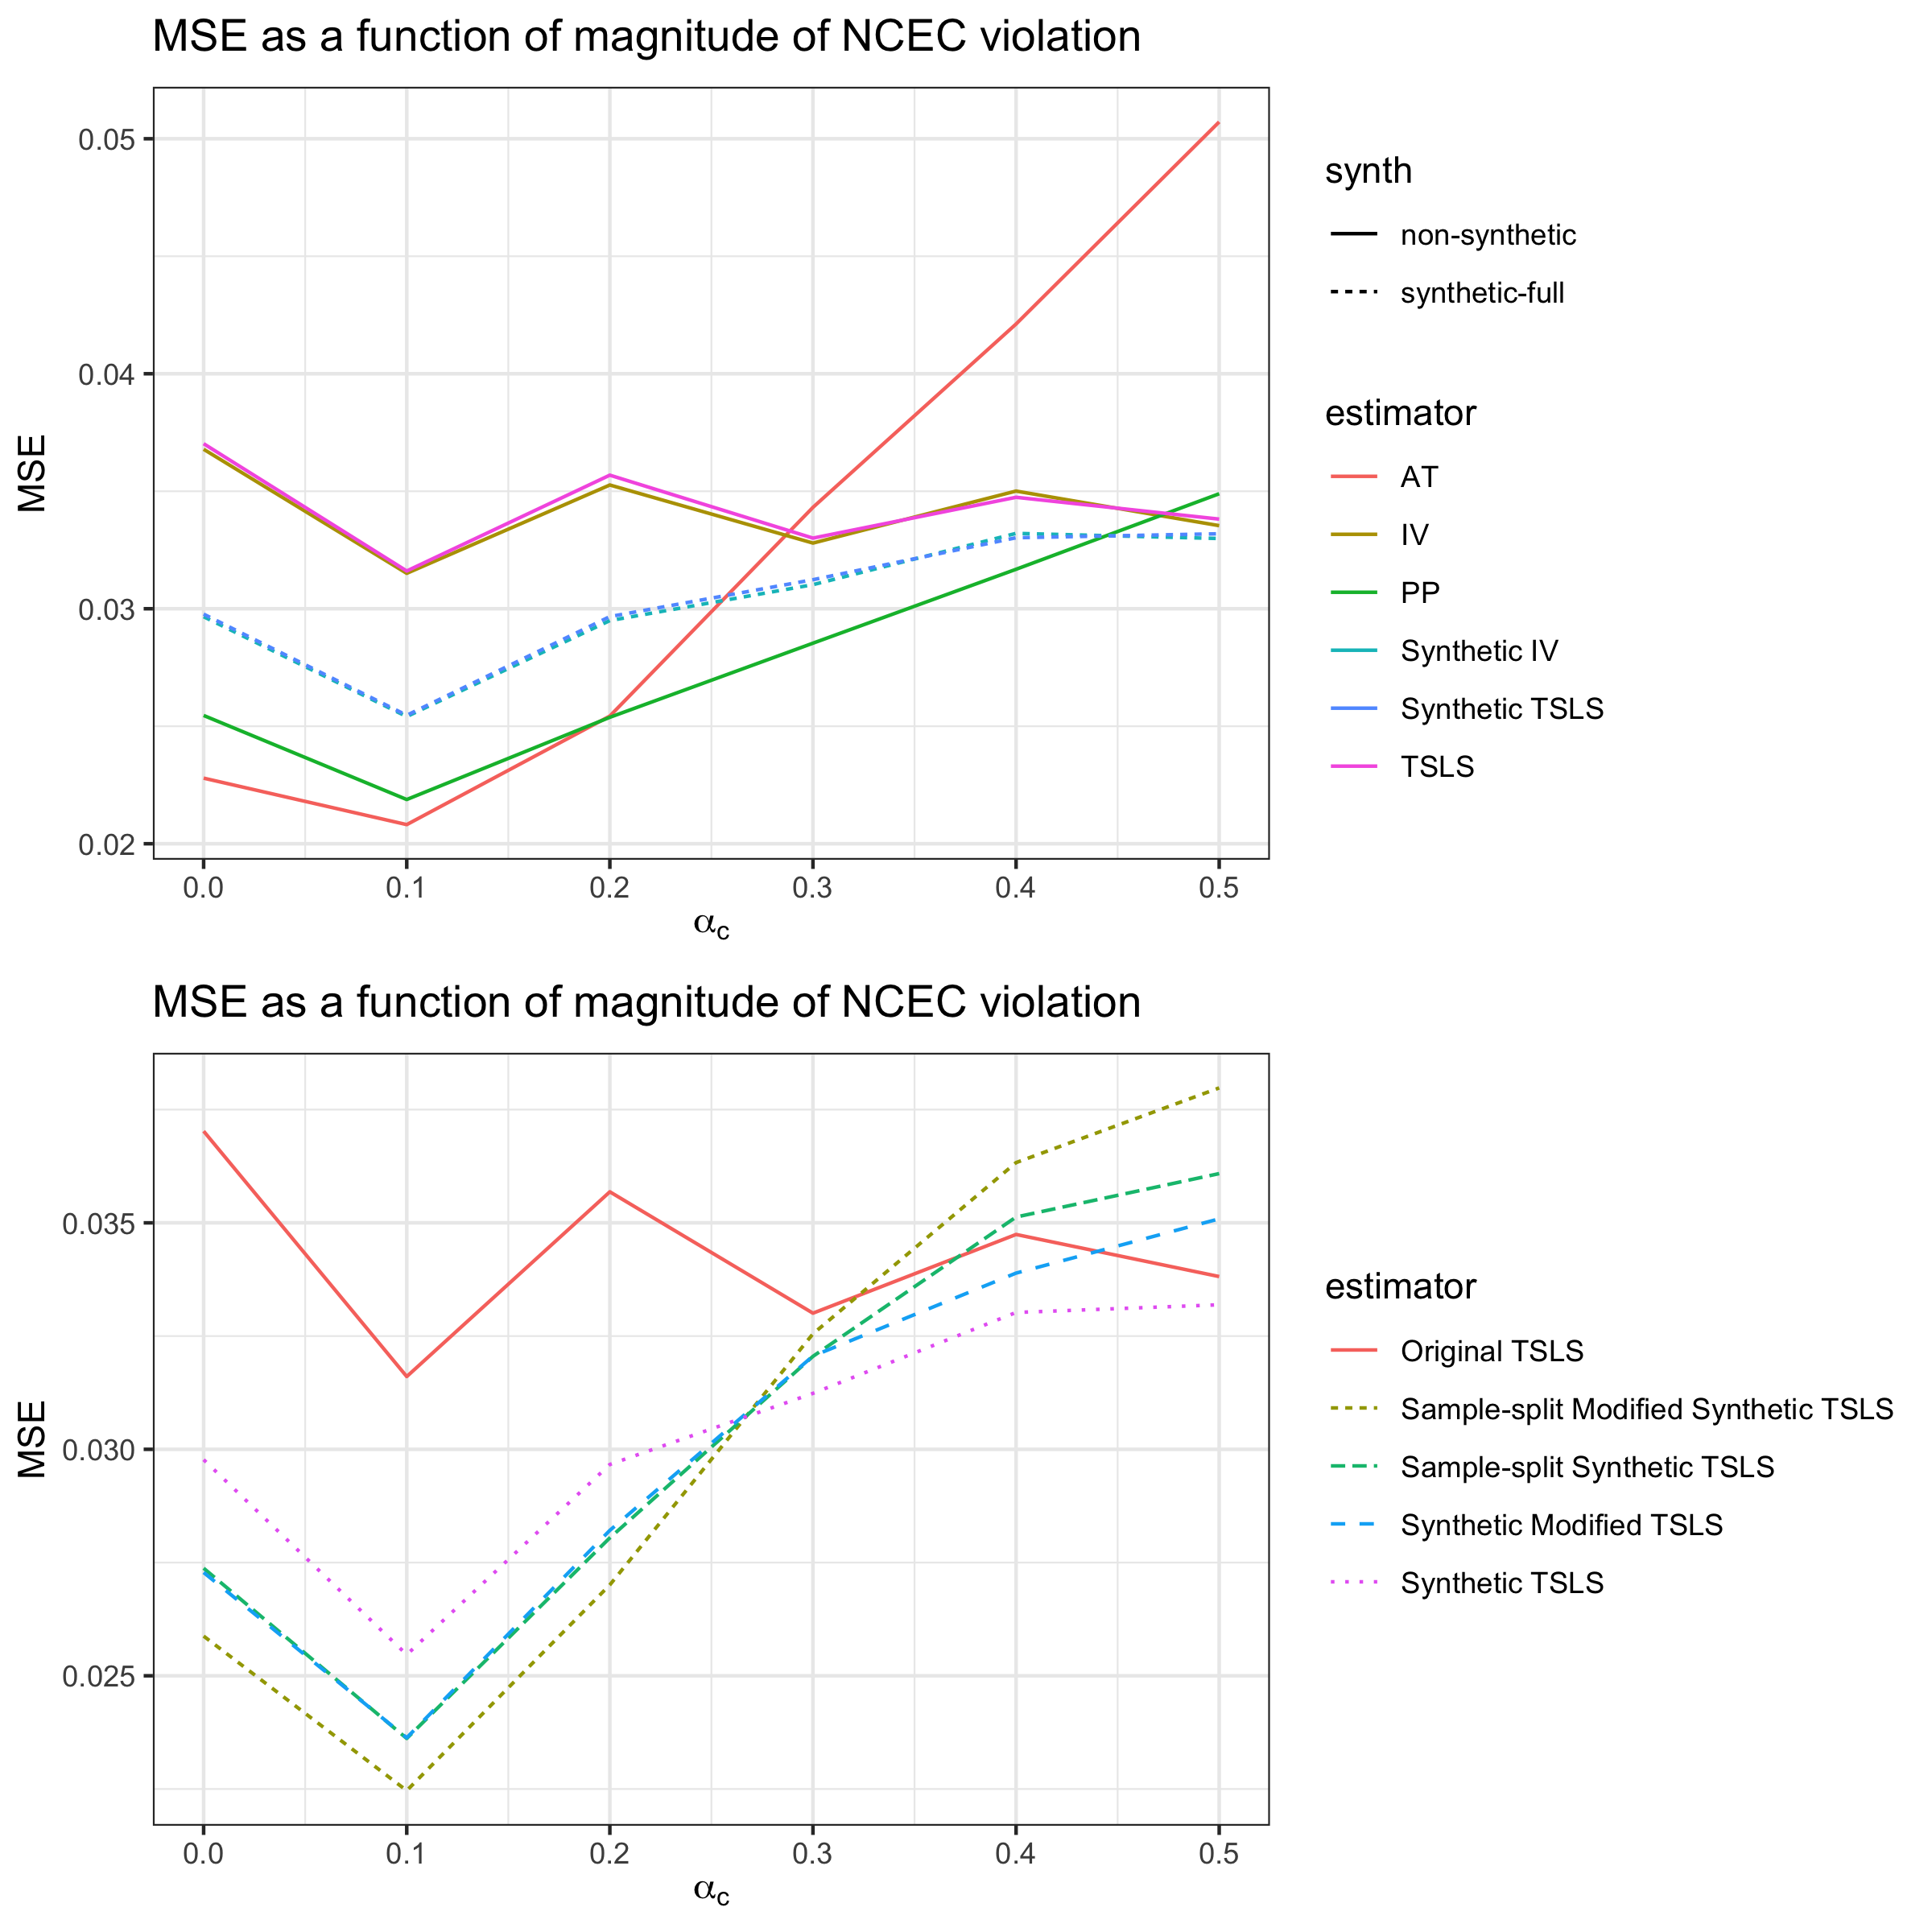
\includegraphics{mse_bias_var_for_n200_cp06.png}
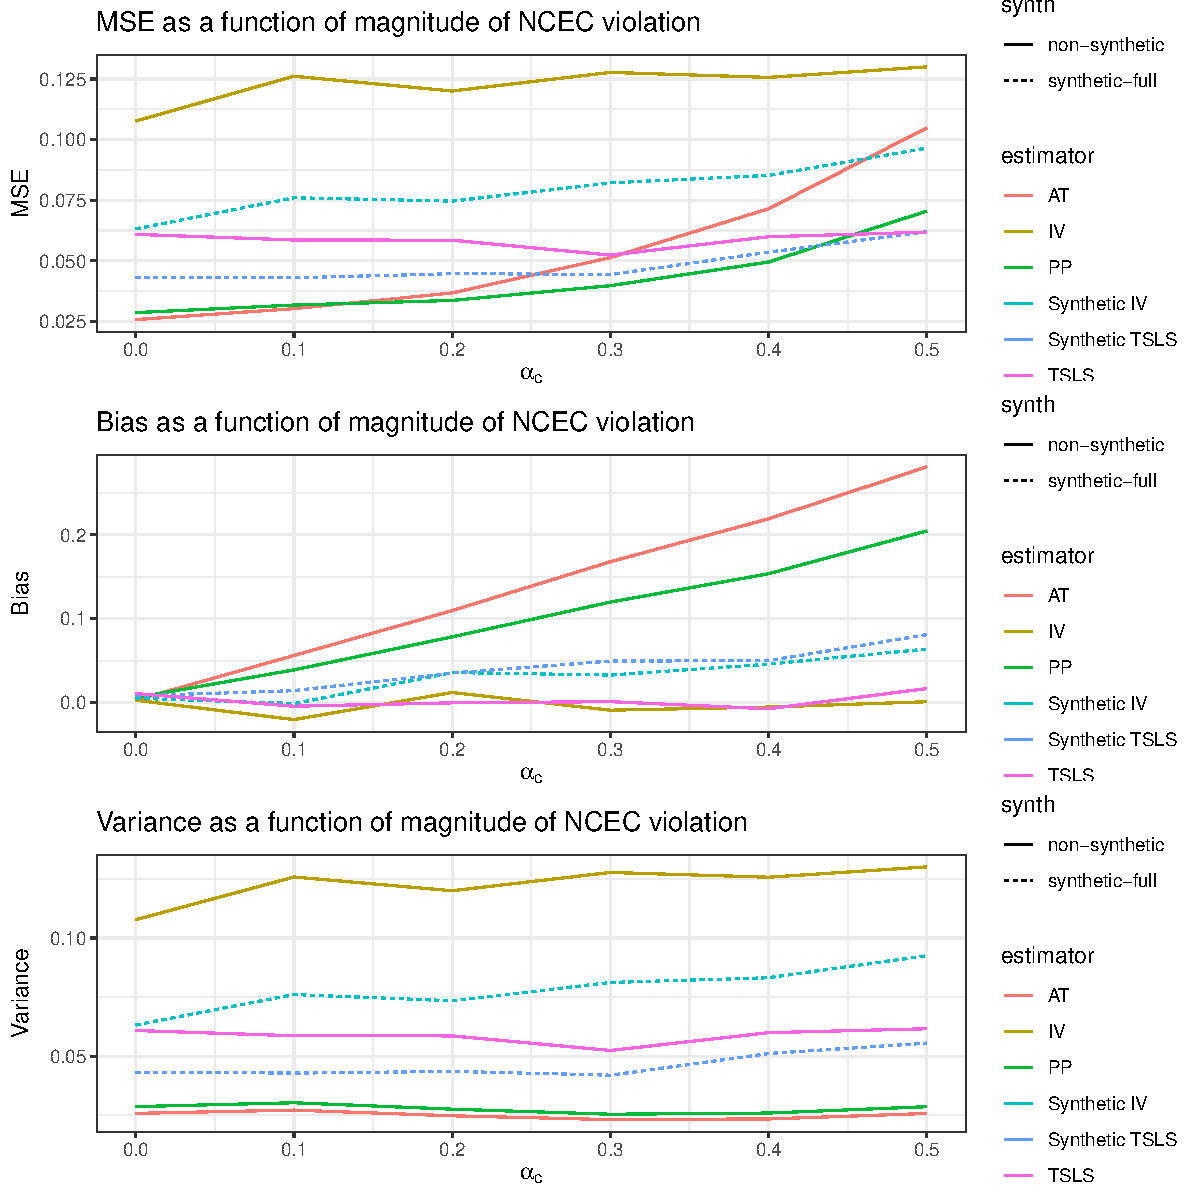
\includegraphics[width =\textwidth]{figures/synthetic-vs-others-plot.pdf}
\end{tabular}\vspace{0.2in}
\caption{MSE, bias, and variance of the four candidate estimators and the two synthetic estimators as $\alpha_c$ changes. The sample size is $n = 200$, and the rest of the parameters are set to $\gamma_c = 0, \lambda_n = \lambda_c = 1, \beta_0 = 0.41, \beta_1 = 2$.}\label{mse_plot_1}
\end{figure}
%
The figure demonstrates that the synthetic estimator has a robustness property. When $\alpha_c$ is low the AT/PP estimators have the lowest MSE, but when $\alpha_c$ grows, the TSLS estimator begins to outperform them, while the IV estimator is always the worst because of its high variance. We see that theh Synthetic IV estimator always improves on the IV estimator in these settings by dramatically reducing its variance. The Synthetic TSLS estimator similarly improves on the TSLS estimator when AT/PP have low bias, but as they incur more and more bias, the performance of the Synthetic TSLS begins to mimic that of the TSLS estimator. 

\begin{figure}
\centering
\begin{tabular}{c}
%\includegraphics{figure_1_correlations.eps}
%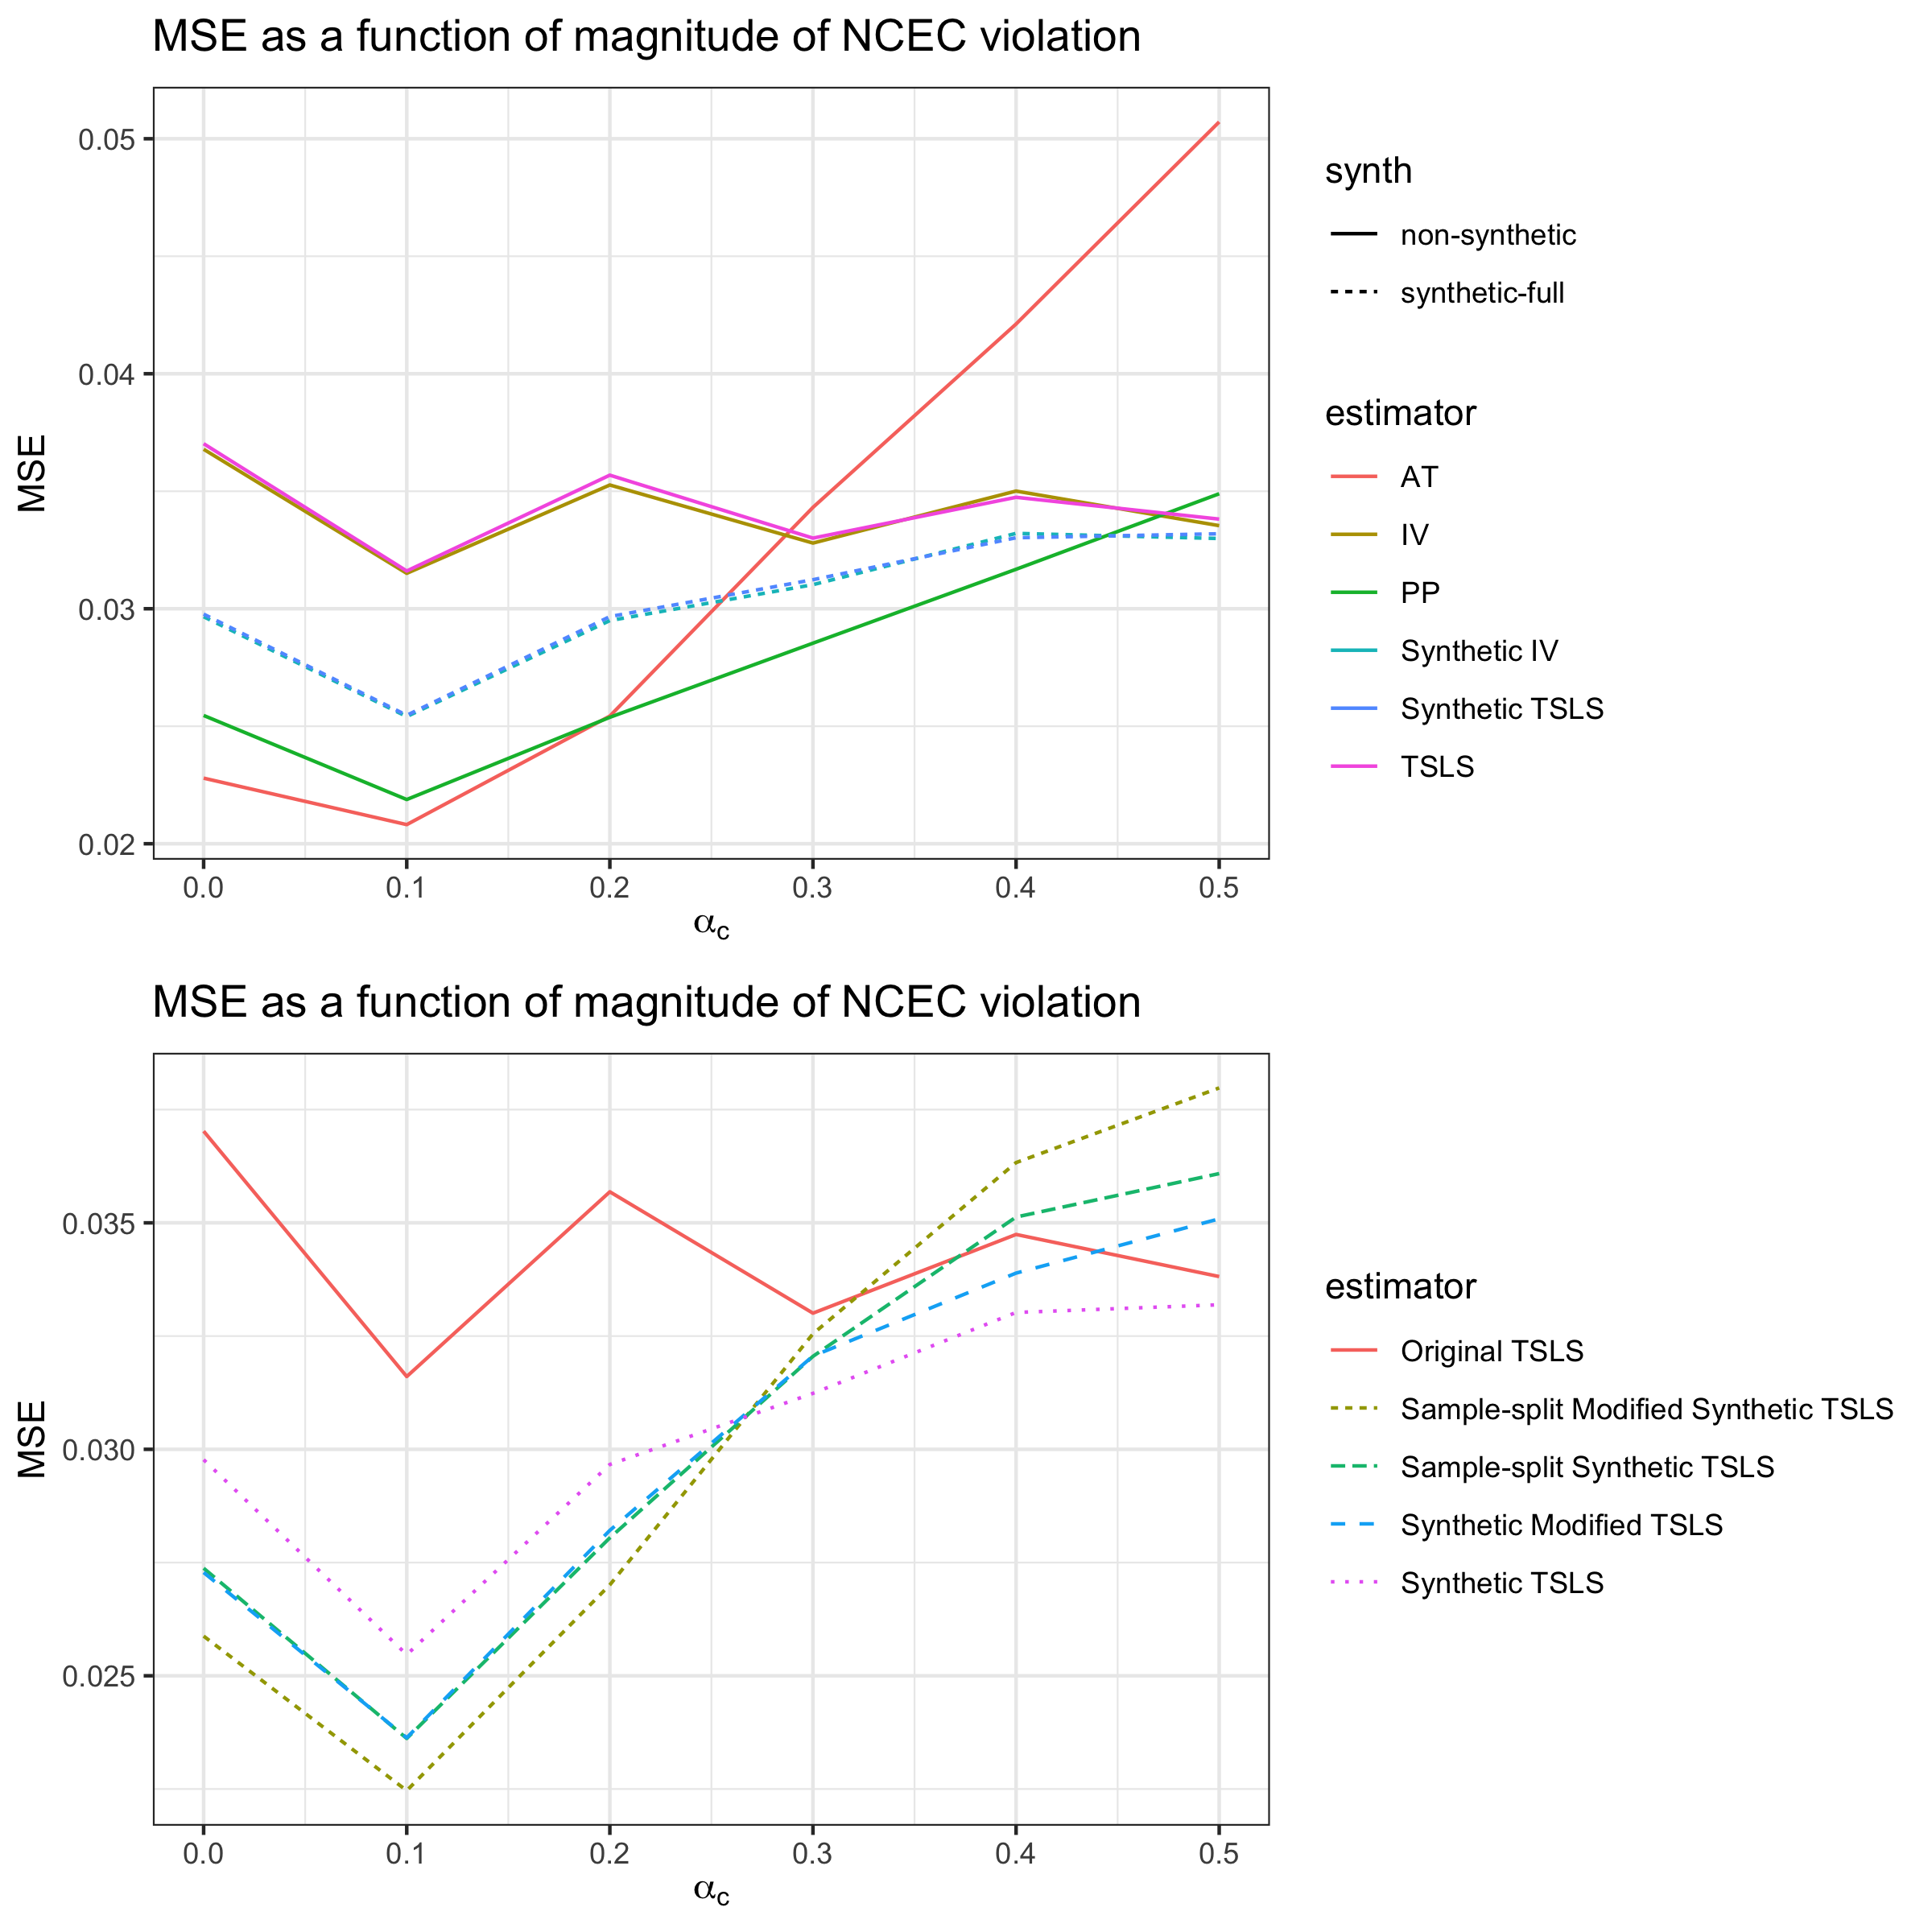
\includegraphics{mse_bias_var_for_n200_cp06.png}
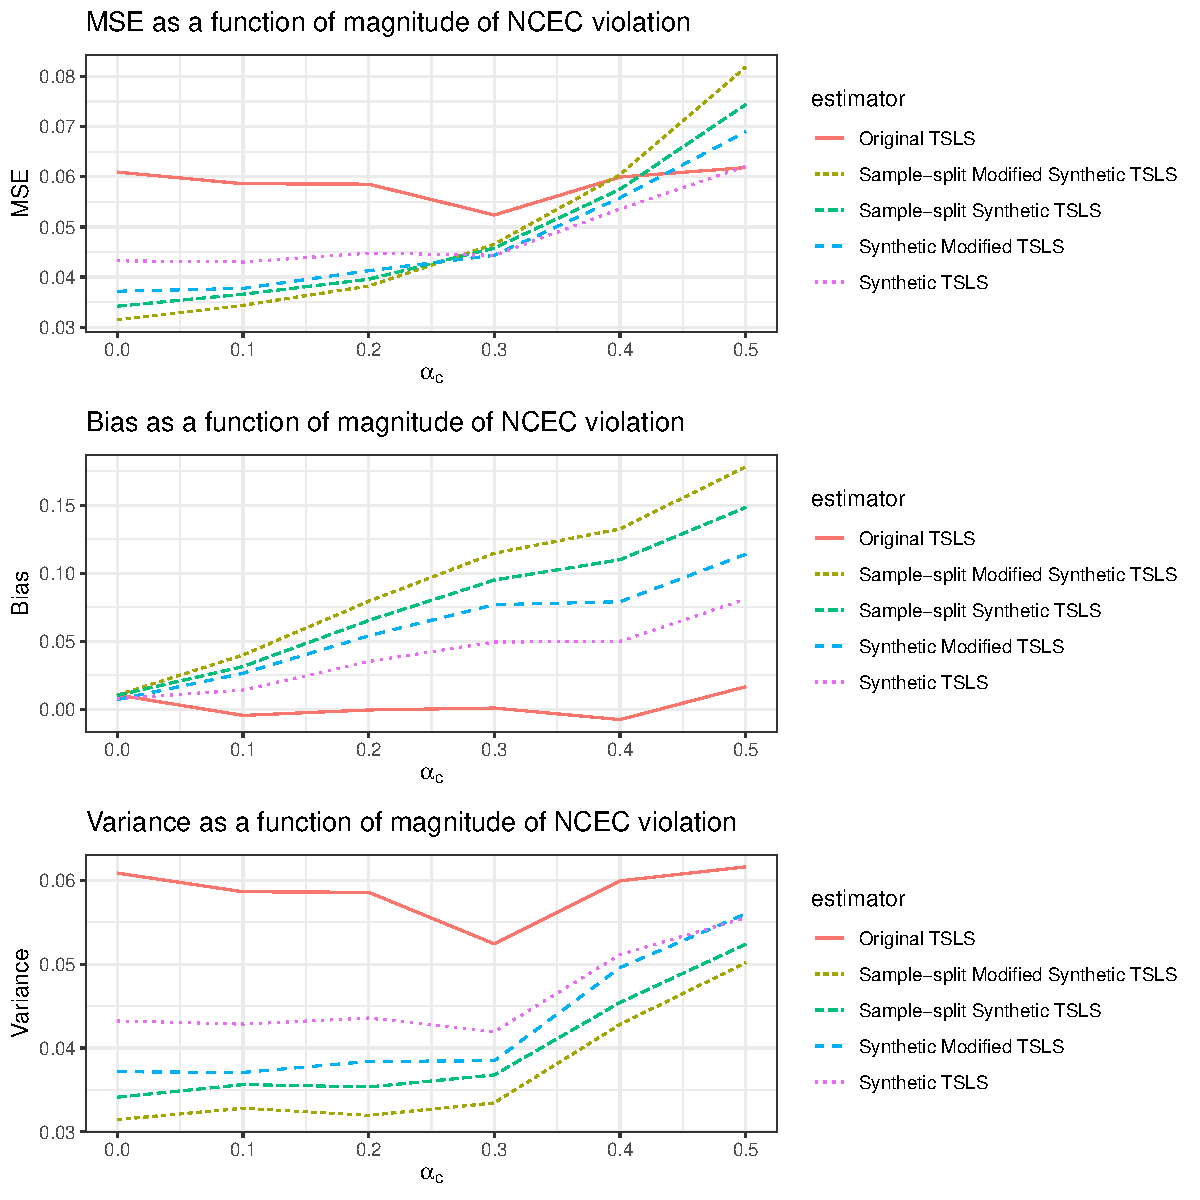
\includegraphics[width =\textwidth]{figures/synthetics-compare-plot.pdf}
\end{tabular}\vspace{0.2in}
\caption{MSE, bias, and variance of the synthetic estimators using different estimates of the bias $\bDelta$, compared to the base TSLS estimator. The sample size is $n = 200$, and the rest of the parameters are set to $\gamma_c = 0, \lambda_n = \lambda_c = 1, \beta_0 = 0.41, \beta_1 = 2$.}\label{mse_plot_2}
\end{figure}
%
The performance of the sample-split and modified raw difference synthetic estimators is demonstrated for the same settings in Figure \ref{mse_plot_2}. In the figure, the estimators using alternative approaches for the bias unsurprisingly have performance that follows a similar trajectory to the Synthetic TSLS. The figure shows that the alternative approaches, by attenuating bias estimates, allow the synthetic estimator to drift farther from the base TSLS estimator: when the AT/PP estimators are best, the alternative approaches benefit more from the good performance of AT/PP than the Synthetic TSLS. On the other hand, when the AT/PP estimators are biased, the alternative approaches are more sensitive to them and acquires a higher MSE compared to the Synthetic TSLS. We see the same behavior in all simulation settings: the synthetic estimator benefits when the AT/PP estimators are best, while taking a small hit in performance when AT/PP are much worse. See for example Figure \ref{mse_plot_3}.

\begin{figure}
\centering
\begin{tabular}{c}
%\includegraphics{figure_1_correlations.eps}
%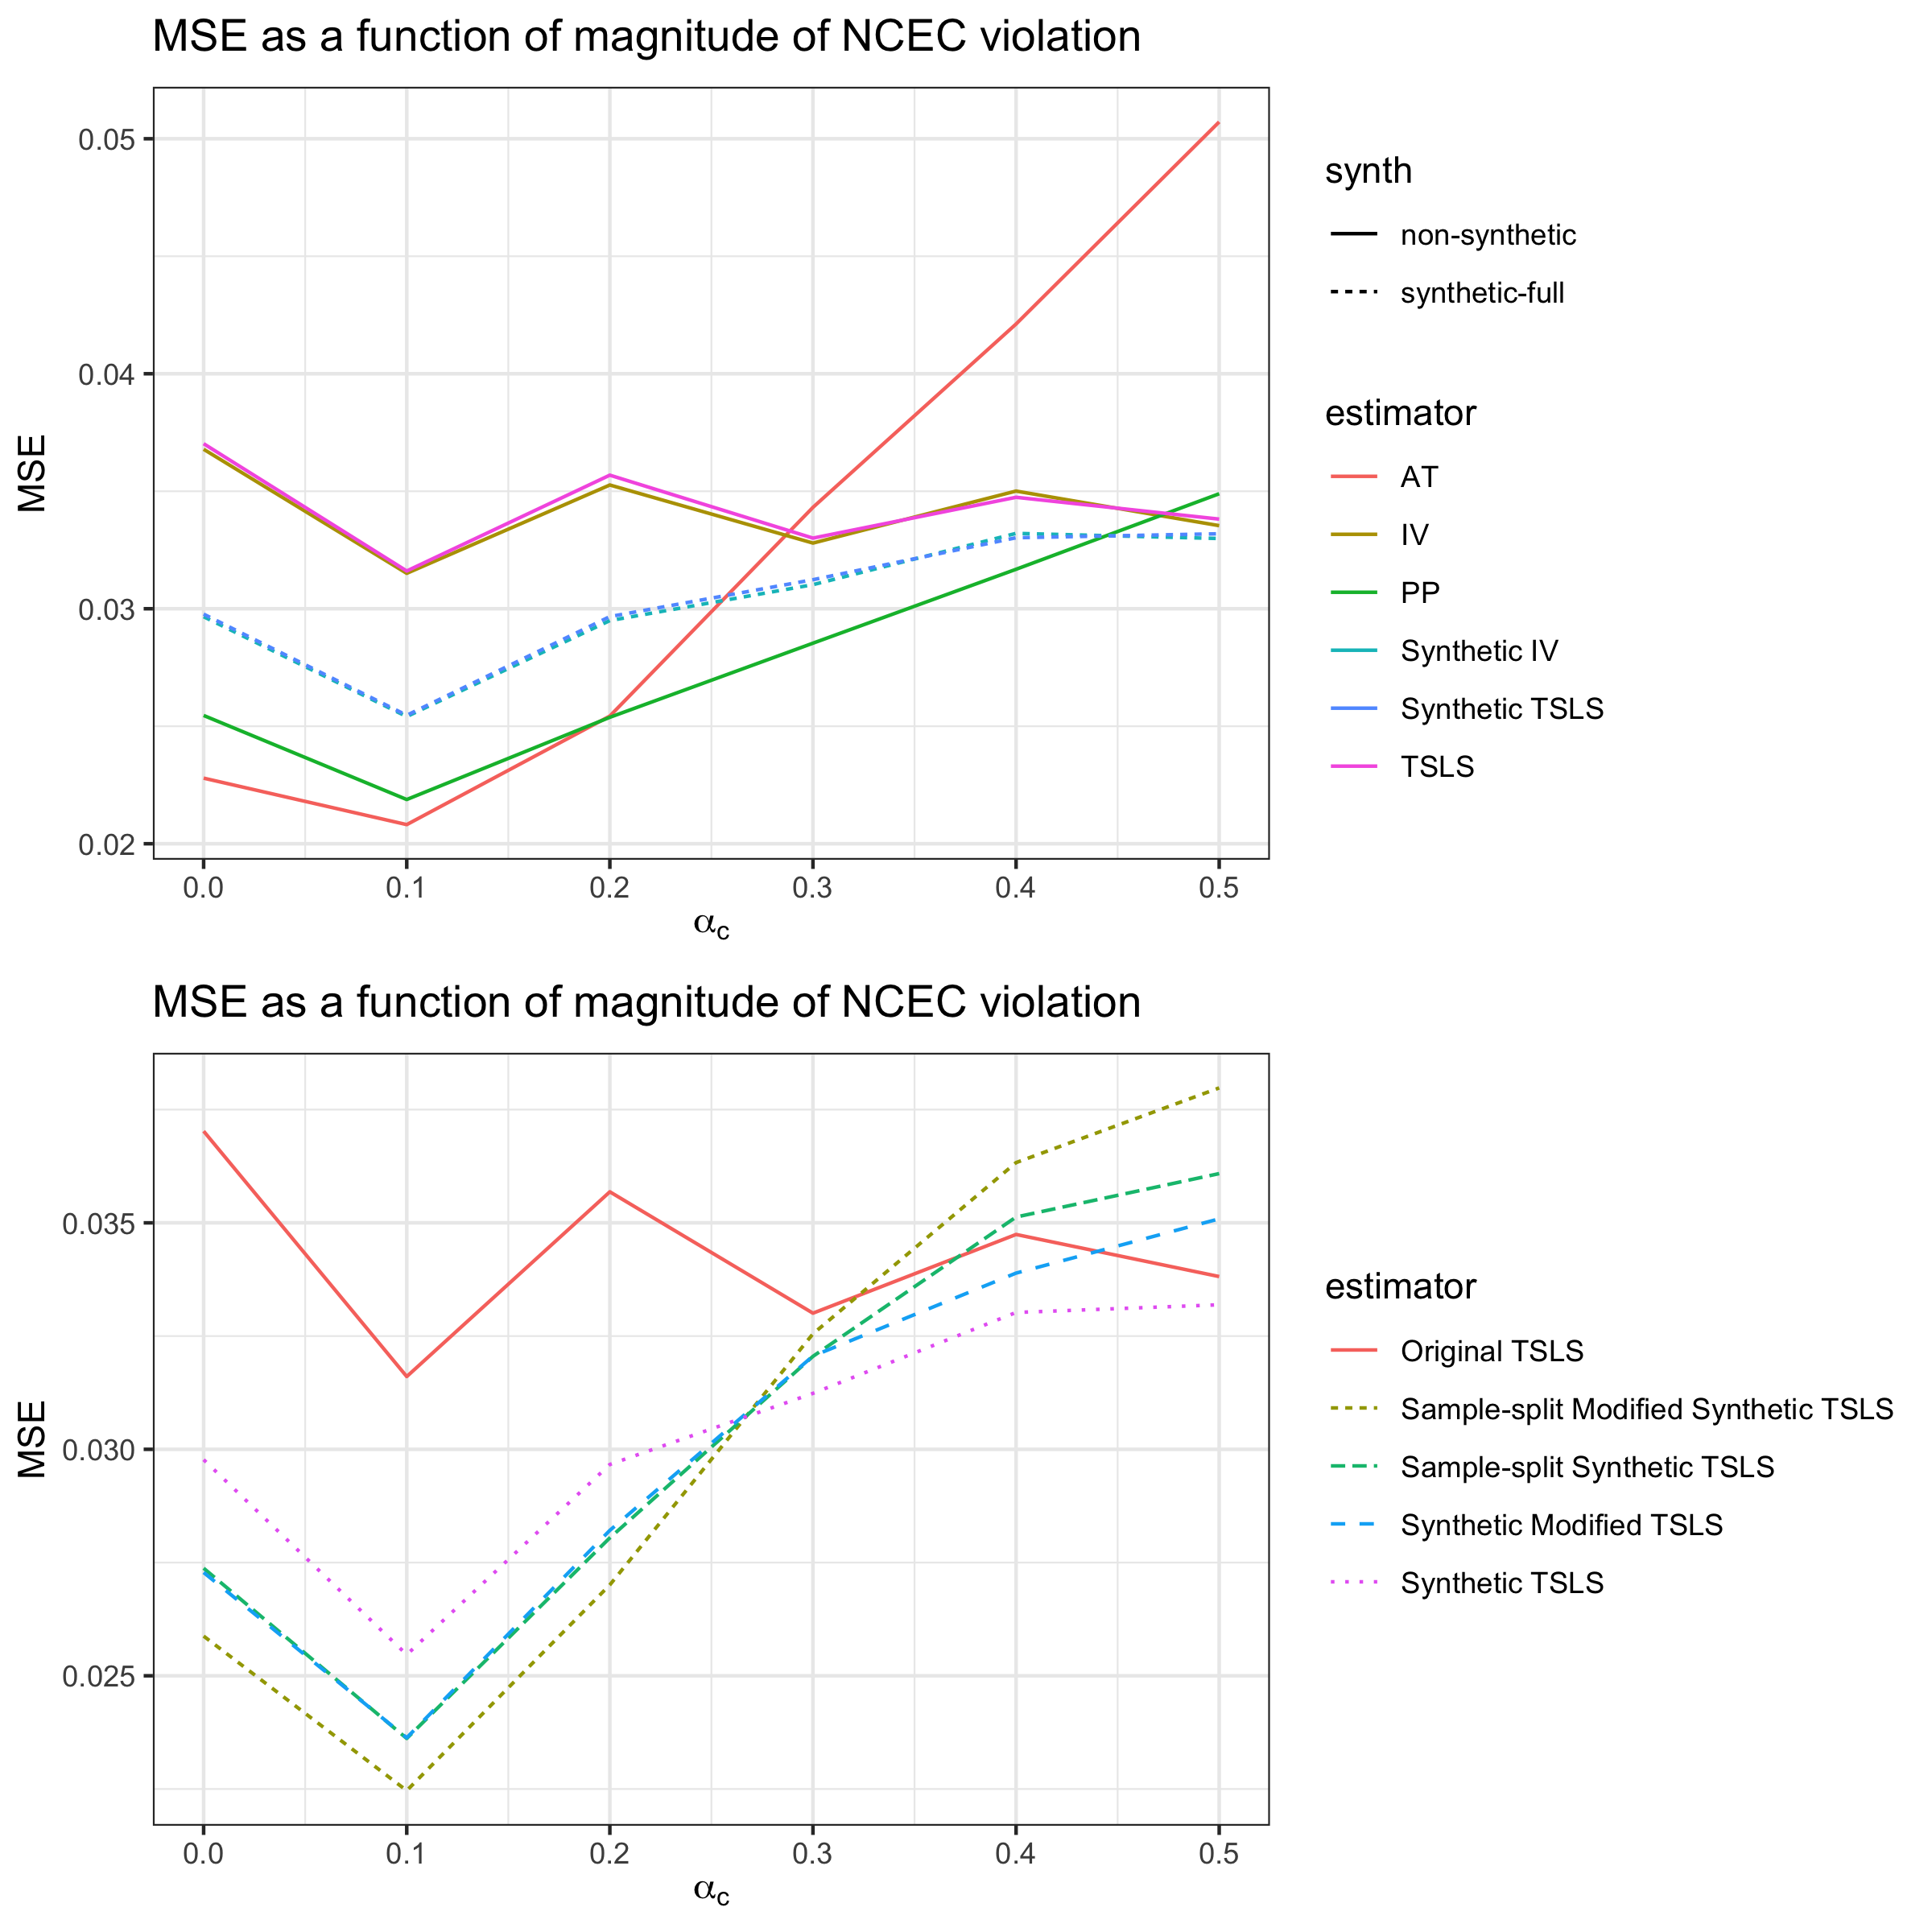
\includegraphics{mse_bias_var_for_n200_cp06.png}
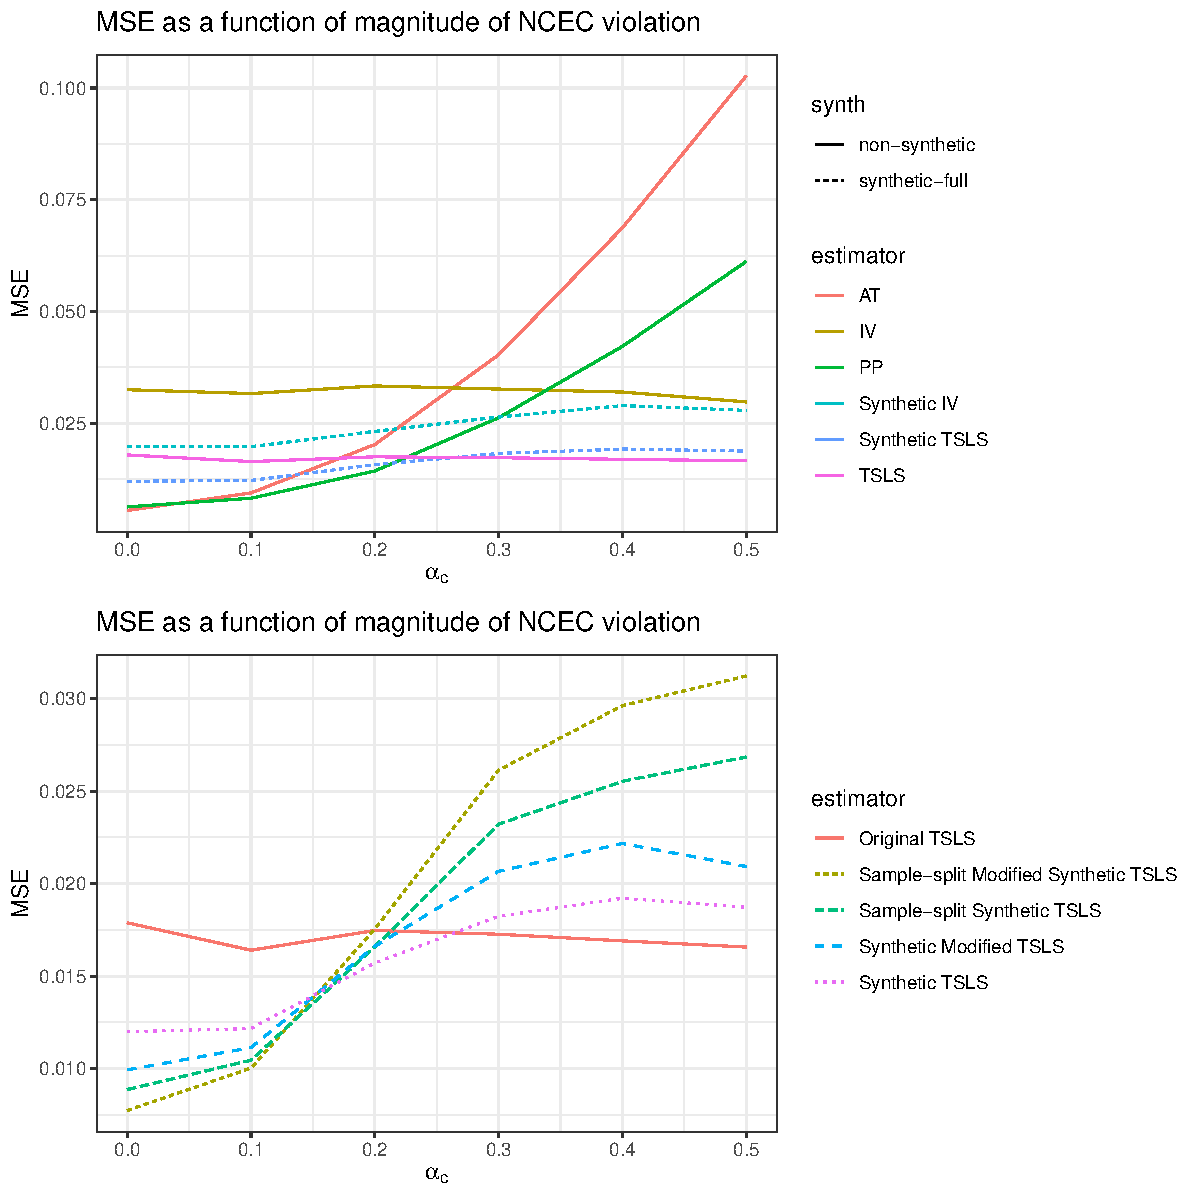
\includegraphics[width =\textwidth]{figures/additional-mse-plot.pdf}
\end{tabular}\vspace{0.2in}
\caption{MSE comparing the Synthetic TSLS estimator to other candidate estimators (top panel); and MSE comparing alternative approaches for bias estimation (bottom panel). The sample size is $n = 1000$, and the rest of the parameters are set to $\gamma_c = 0, \lambda_n = \lambda_c = 1, \beta_0 = 0.41, \beta_1 = 0.5$.}\label{mse_plot_3}
\end{figure}

\bibliography{compliance_refs}
\bibliographystyle{unsrtnat}

\end{document}

%\theta\right\}\sum_{j=1}^5\tdot_j(\bgamma_n)(\bgammahat_{nj} - \bgamma_{nj})\right],
%\] \\
%\end{split}\end{equation}
%\end{document}

